% Rackham Style Guide and Tempalte -  https://rackham.umich.edu/wp-content/uploads/2020/09/dissertation-handbook.pdf
% Mia Stevens Thesis - https://deepblue.lib.umich.edu/bitstream/handle/2027.42/153391/minist_1.pdf?sequence=1
\documentclass[thesis]{./style/thesis-umich}

% Used to allow authors name to be repeated in bibliography. IEEE citation style. Also need a command on first line of .bbl file
% \usepackage[redeflists]{IEEEtrantools}
\usepackage{booktabs}
\usepackage{subcaption}
\usepackage{enumitem}
\usepackage{amsmath}
\usepackage{mathtools}
\DeclareMathOperator*{\argminA}{arg\,min}

\title{Mapping and Real-time Navigation \\ with application to Small UAS Urgent Landing}

% Author name
\author{Jeremy D. Castagno}
\authoremail{jdcasta@umich.edu}
\orcidid{0000-0001-5458-9787}

% Department
\department{Robotics}

% Year of completion
\year=2021

% \dedication{
%   This manual is dedicated to my family.
% }

% \acknowledgments{
%   .
% }

% \preface{
%   This disseration is a sample document using the \texttt{thesis-umich.cls}
%   template.
% }

\committee{
  Professor Ella Atkins, Chair,\\
  Professor Nadine Sarter, \\
  Assistant Professor Maani Ghaffari Jadidi, \\
  Professor Quentin Stout
}


% Definition of any abbreviations used.
\acronyms{
 \acro{AGL}{Above Ground Level}
 \acro{AHC}{Agglomerative Hierarchical Clustering}
 \acro{CNN}{Convolutional Neural Networks}
 \acro{CRS}{Coordinate Reference System}
 \acro{DSM}{Digital Surface Model}
 \acro{ECAL}{Enhanced Communication and Abstraction Library}
 \acro{FAA}{Federal Aviation Administration}
 \acro{GIS}{Geographic Information System}
 \acro{GPS}{Global Positioning System}
 \acro{GPU}{Graphics Processing Unit}
 \acro{GCS}{Geographic Coordinate System}
 \acro{INS}{Inertial Navigation System}
 \acro{IOU}{Intersection over Union}
 \acro{LiDAR}{Light Detection and Ranging}
 \acro{MSL}{Mean Sea Level}
 \acro{MCS}{Motion Capture System}
 \acro{OPC}{Organized Point Cloud}
 \acro{OGC}{Open Geospatial Consortium}
 \acro{OSM}{Open Street Map}
 \acro{PIC}{Pilot in Command}
 \acro{RGB}{Red Green Blue}
 \acro{RGBD}{Red Green Blue Depth}
 \acro{SfM}{Structure from Motion}
 \acro{SVM}{Support Vector Machines}
 \acro{SBC}{Single Board Computer}
 \acro{TSDF}{Truncated Signed Distance Function}
 \acro{UAS}{Unmanned Aircraft Systems}
%  \acro{UTM}{Universal Transverse Mercator}
 \acro{UTM}{UAS Traffic Management}
 \acro{sUAS}{small Unmanned Aircraft Systems}
 \acro{VTOL}{Vertical Take-of and Landing}
 \acro{VR}{Virtual Reality}
}

% Commands to hide or show lists of figures, tables, etc.
%\showlistoffigures
%\showlistoftables
%\showlistofmaps
%\showlistofillustrations
% \showlistofappendices
% \showlistofabbreviations
% \showlistofacronyms
%\showlistofsymbos
% OR
\hidelistoffigures
\hidelistoftables
\hidelistofmaps
\hidelistofillustrations
\hidelistofappendices
\hidelistofabbreviations
\hidelistofacronyms
\hidelistofsymbols

% Definition of any abbreviations used.
%\abbreviations{
% \acro{LS&A}{Literature Science and Arts}
%}


% Some abstract text
% \abstract{
%   Write abstract here
% }

\begin{document}

% Used to allow authors name to be repeated in bibliography. IEEE citation style. Also need a command on first line of .bbl file
% \bstctlcite{IEEEexample:BSTcontrol}

\chapter{Introduction}
 \label{ch:introduction}
 
\paragraph{Motivation}

Unmanned Aircraft System (UAS) are expected to proliferate in low-altitude airspace over the coming decade. Drones with vertical takeoff and landing (VTOL) capability have been proposed to offer fast package delivery, monitor and secure assets, perform inspections, and entertain.
% The \acf{FAA} estimates over 1.25 million \acf{sUAS} were flown in 2018 \cite{federal_aviation_administration_unmanned_2019}, far exceeding the number of registered manned aircraft in the USA.  Many \ac{sUAS} are  configured for \acf{VTOL} because of requirements for minimal area for ingress and egress in cities.  
Low-altitude operation of UAS in urban areas will require flight near buildings and over people. 
% Safety must be a top priority for system designers and regulators as UAS will pose new risks to the overflown population.
A primary safety concern is ensuring a robust urgent landing capability \cite{winnefeld_unmanned_2011,degarmo_issues_2013}.  Urgent landing requires landing site selection, trajectory planning, and stable flight control to actually reach the selected site \cite{atkins_emergency_2006}. It is possible a UAS may identify a safe site within sensor range allowing for an immediate landing.  However, when no safe site is within range the UAS must devote time and energy to exploring sites beyond sensor range or else utilize pre-processed data to identify a safe site \cite{ten_harmsel_emergency_2017,ochoa_fail-safe_2017}.  An onboard database of maps including landing sites can be incorporated into an efficient autonomous decision making framework \cite{sankararaman_towards_2017}. Offline data sources such as satellite images, airborne LiDAR point clouds, and existing map data may be used to aid map construction.
% Such a framework should incorporate risk models which account for both the intrinsic risk of the landing site as well as the path risk to reach the landing site.
% For example, Refs.  \cite{atkins_emergency_2006, meuleau_emergency_2009}  and \cite{sankararaman_towards_2017} utilize airborne flight risk models to build emergency landing plans for fixed-wing and urban flight operations, respectively. We call such a decision making framework a map-based planner.

Conventional fixed-wing emergency landing sites such as open fields and roadways are either extremely rare or highly populated in and around cities. Consider the satellite image in Figure \ref{fig:ch1_challenge_urban} which shows the typical sparsity of conventional landing zones in the city Witten, Germany. However, these images show a multitude of unoccupied flat rooftops that may provide nearby landing sites for small lightweight UAS. Obstacles such as air conditioning units, skylights, and rooftop entrances on these surfaces may be present and must be explicitly modeled and avoided during an urgent landing. Polygons can accurately and simply represent these flat surfaces as well as obstacles embedded on them per Figure \ref{fig:ch1_roof_shape_obstacle}. Archived data can be processed such that rooftop landing sites substantially augment existing conventional landing site databases.






% \acf{GIS} use polygons in vector map data to represent many items such as parks, fields, and buildings outlines. 
% This dissertation will have a strong focus on creating databases of such flat surfaces using efficient computational geometry routines coupled with deep learning.  


% \begin{figure}[ht]
%     \centering
%     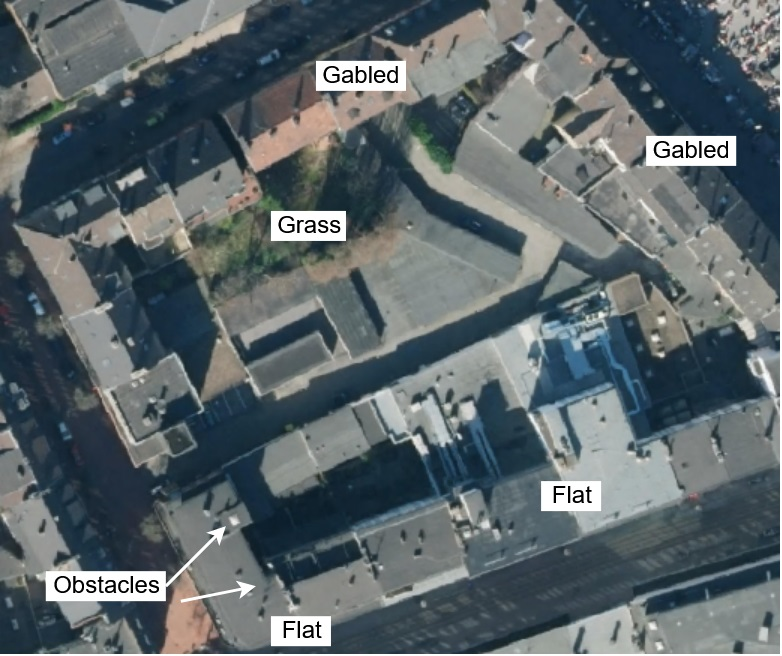
\includegraphics[clip, trim=0.0cm 0cm 0cm 0cm, width=0.55\linewidth]{chapter_5_mapping/imgs/challenge_urban-Page-2.jpg}
%     \caption{Satellite image of an urban environment with multiple flat roof landing sites. Select roof shapes and obstacles are labeled.}
%     \label{fig:ch1_challenge_urban}
% \end{figure}


\begin{figure}[ht]
    \centering
  \begin{subfigure}{.45\linewidth}
    \centering
    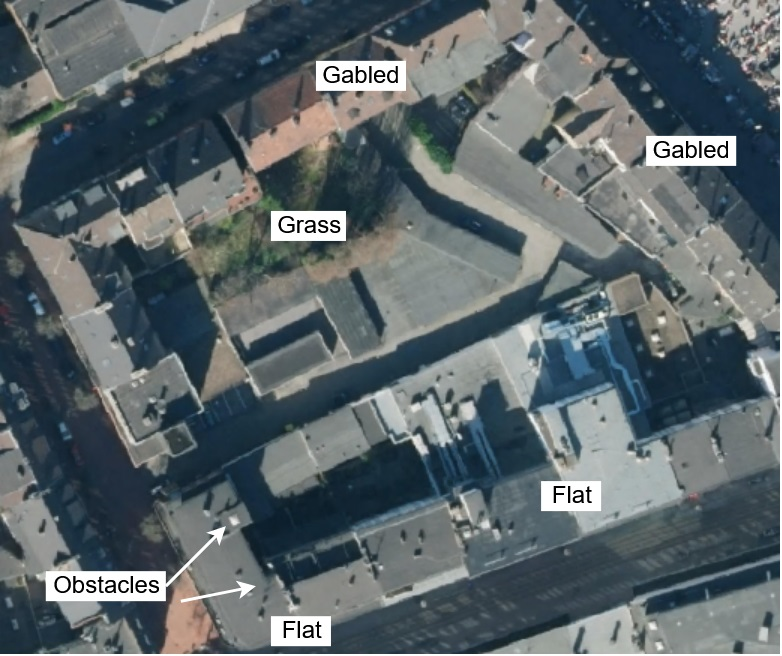
\includegraphics[clip, trim=0.0cm 0cm 0cm 0.55cm, width=0.95\linewidth]{chapter_5_mapping/imgs/challenge_urban-Page-2.jpg}
    \caption{}
    \label{fig:ch1_challenge_urban}
  \end{subfigure}
  \begin{subfigure}{.45\linewidth}
    \centering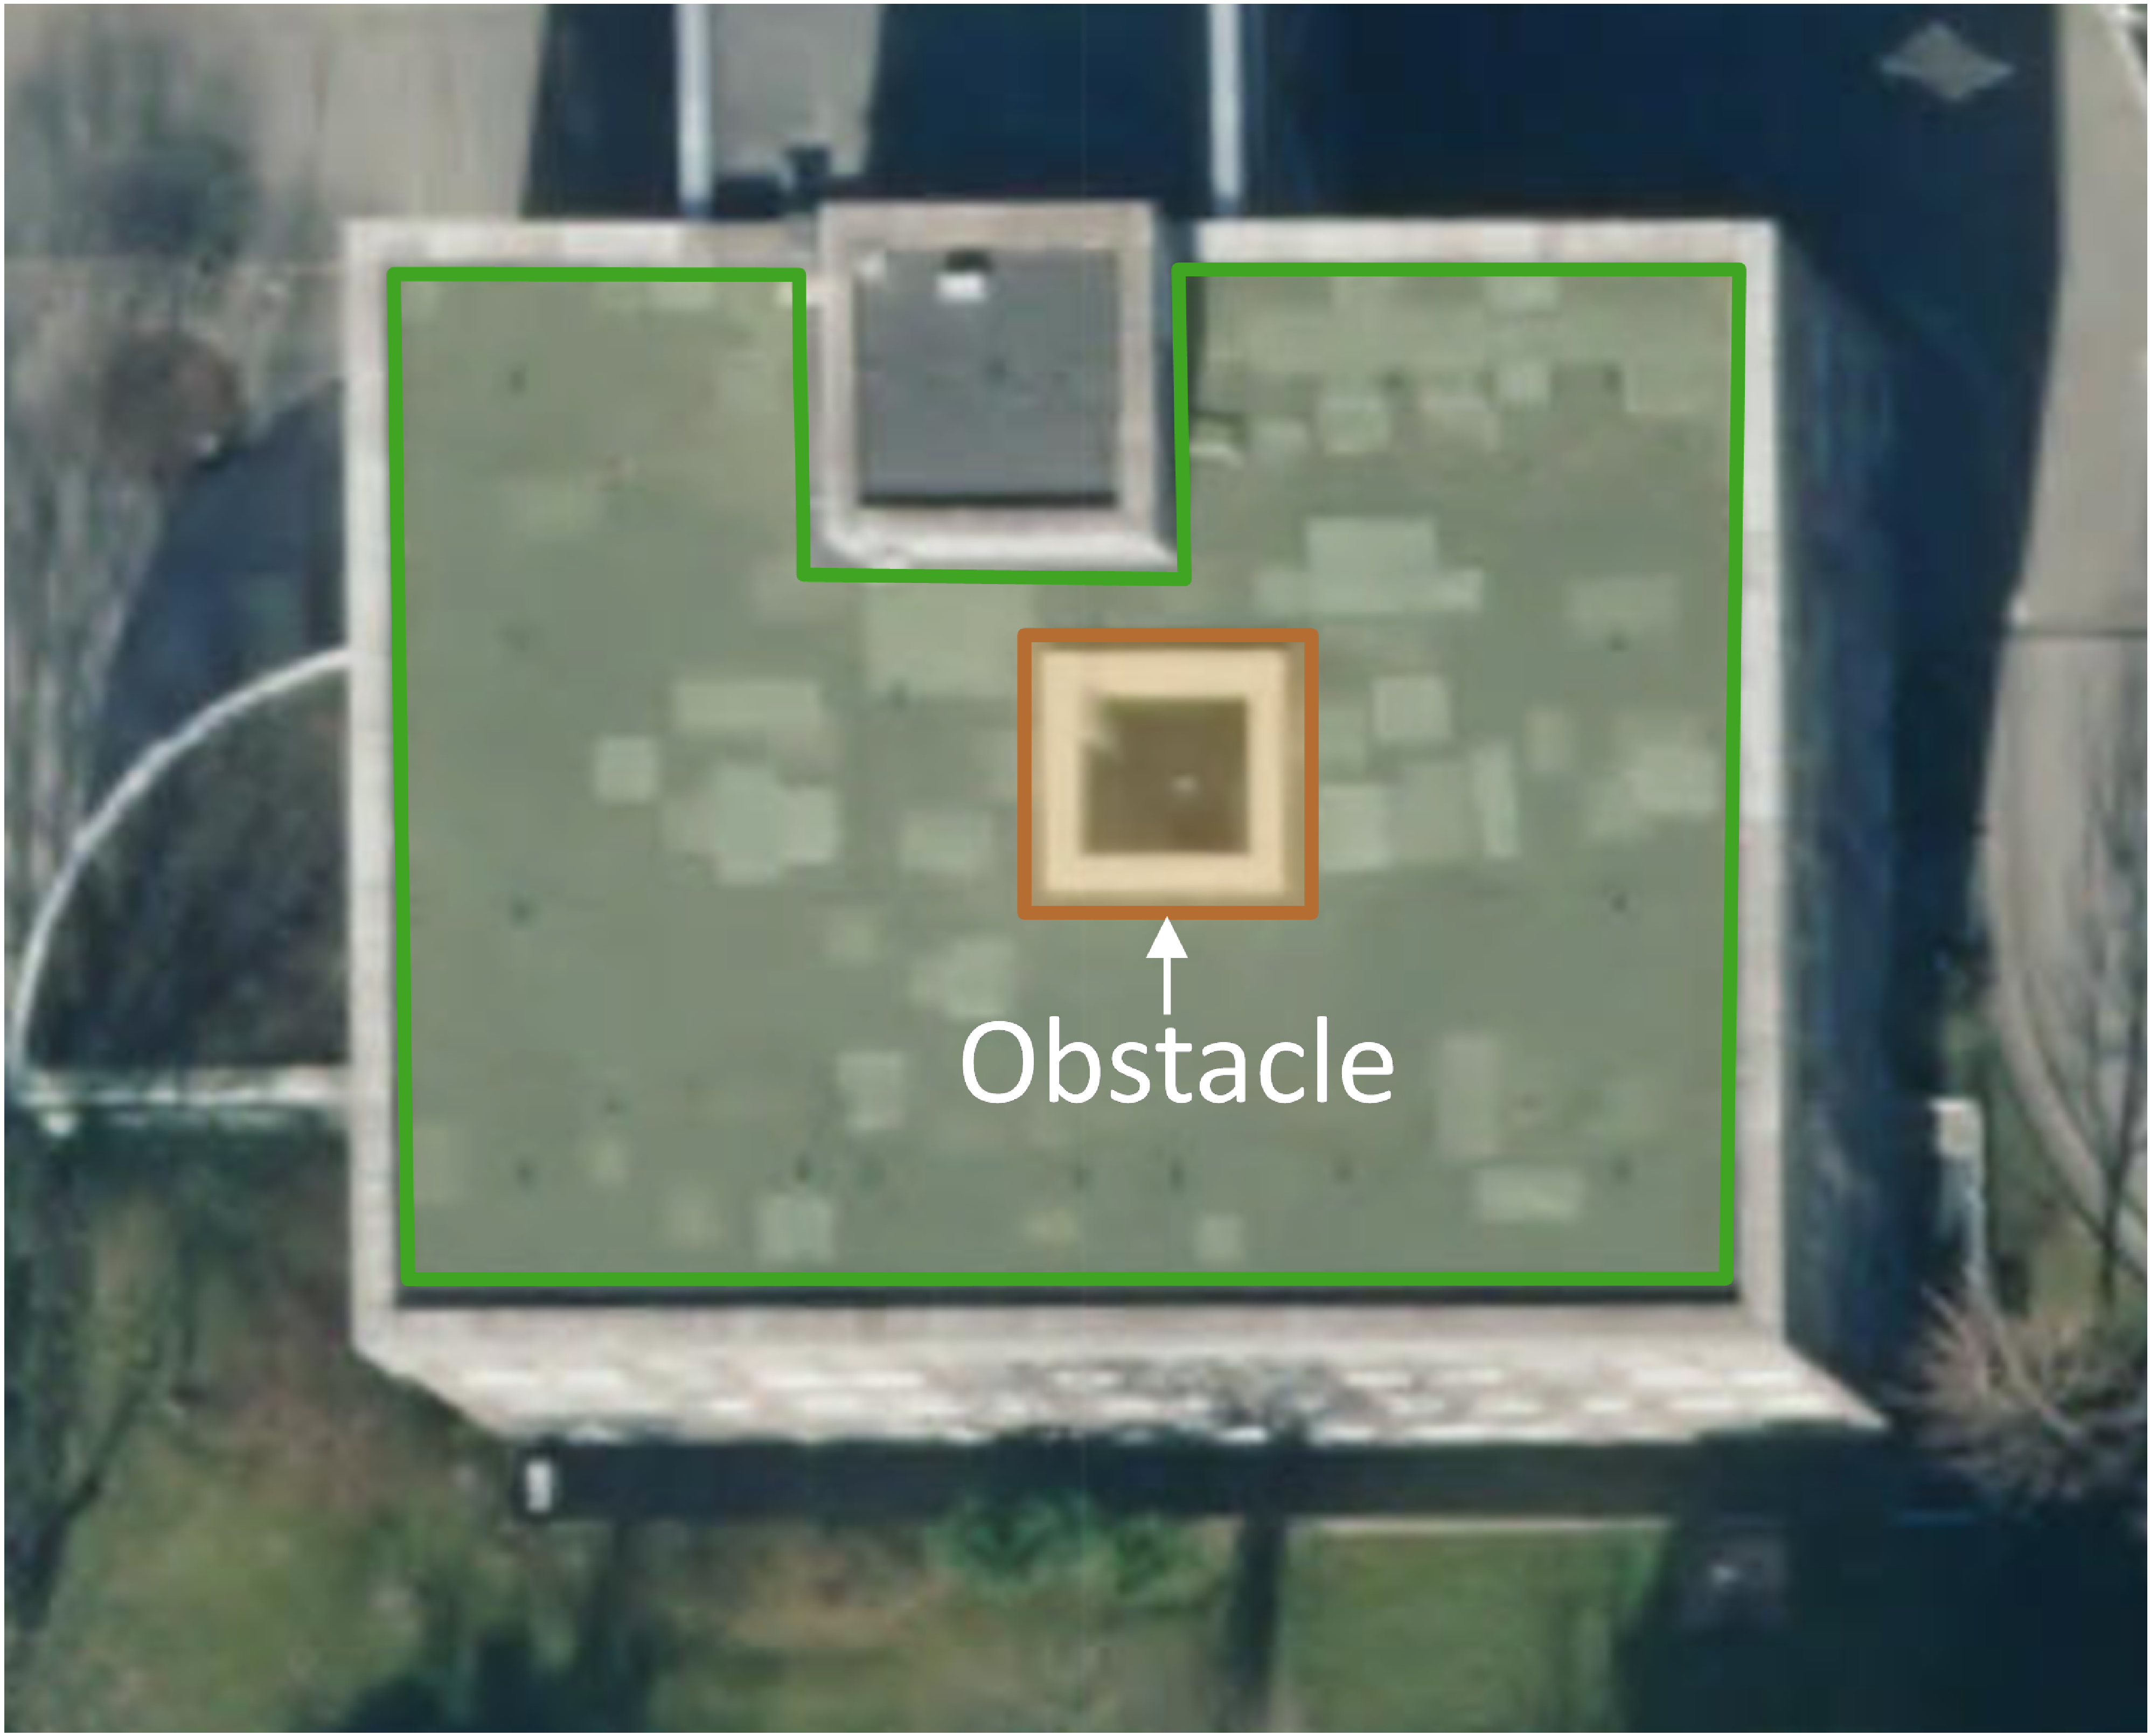
\includegraphics[width=.95\linewidth]{chapter_1_intro/imgs/roof_shape_obstacle.pdf}
    \caption{}
    \label{fig:ch1_roof_shape_obstacle}
  \end{subfigure}
  \caption{(\subref{fig:ch1_challenge_urban}) Satellite image of an urban environment with multiple flat rooftops. Select roof shapes and obstacles are labeled.  (\subref{fig:ch1_roof_shape_obstacle}) A rooftop surface can be represented as a non-convex polygon with an exterior shell (green) and interior hole(s) (orange).  }\label{fig:ch1_motivation}
\end{figure}




\paragraph{Problem Statement}

This dissertation aims to address the following challenges:

\begin{enumerate}[noitemsep]
    \itemsep0em 
    \item Where can a small UAS safely land in a city during an urgent or emergency landing situation?
    \item How can maps be constructed and risk evaluated for landing site selection and path planning?
    % \item What path should it take reach this landing site?
    \item How can the small UAS verify a landing zone is safe in real-time on approach to that site?
\end{enumerate}

Previous research has proposed the use of public Geographic Information Systems (GIS) datasets such as satellite images, airborne LiDAR point clouds, digital elevation maps, census data, and building outlines for terrain-based landing site identification, risk assessment, and path planning \cite{meuleau_emergency_2009, di_donato_evaluating_2017, patterson_timely_2014, bleier_risk_2015}.  However increased use of sUAS in urban cities motivates this work to additionally consider building rooftops as landing sites. To our knowledge this dissertation is the first work to explicitly use GIS data to automatically identify flat rooftop buildings, isolate flat surfaces, and find risk-minimum touchdown points that maximize distance to obstacles. 

% These conventional landing sites are often risk evaluated by terrain type and size \cite{di_donato_evaluating_2017}. 
\paragraph{Research Approach}

% Map data is widely available in vector form, such as polygons, which describes features such as fields, parks, and building outlines \cite{openstreetmap_contributors_planet_2017}.  Such polygons can be efficiently stored and indexed such that spatial queries may efficiently computed in an embedded database \cite{furieri_spatialite_2017}. 

This dissertation proposes to process existing GIS data to extract safe landing sites and occupancy maps used for map-based planning. To accomplishing this several computational geometry algorithms have been developed to enable efficient extraction of flat surfaces as non-convex polygons. The overall structure of this dissertation is shown in Figure \ref{fig:ch1_thesis_overview} and can be summarized as accomplishing the following six tasks:
% This dissertation assumes these urgent landing scenarios are without loss-of-control, for example: low battery energy, lost communication link, adverse weather, non-essential sensor or actuator failure, operator emergency landing directive, and non-cooperative aircraft nearby.

\begin{enumerate}[noitemsep]
    \item Efficiently extract non-convex polygons with interior holes from 2D point sets. (Ch. 2)
    \item Extend polygon extraction methods from 2D point sets to 3D data where polygons represent flat surfaces and interior holes represent obstacles embedded on the surface. (Ch. 3)
    \item Classify rooftop shape in a city (e.g., flat) with high confidence in model prediction. (Ch. 4)
    \item Assimilate publicly available GIS data such as satellite images, airborne LiDAR point clouds, and existing map data into an urgent landing site database with associated risk metrics as well as occupancy maps for path planning. (Ch. 5)
    \item Create a multi-goal planner to efficiently search through candidate sites and account for landing site risk as well as flight path risk to that site. The planner identifies a landing site/path pair to minimize combined \emph{total} risk as well as computation time for this search. (Ch. 5)
    \item Perform experiments to verify the planned touchdown location is safe in real-time using on-board sensors such as LiDAR. (Ch. 6, Proposed)
\end{enumerate}

% The final risk-optimal landing site/path pair is sent to a navigation controller.
\begin{figure}[t]
    \centering
    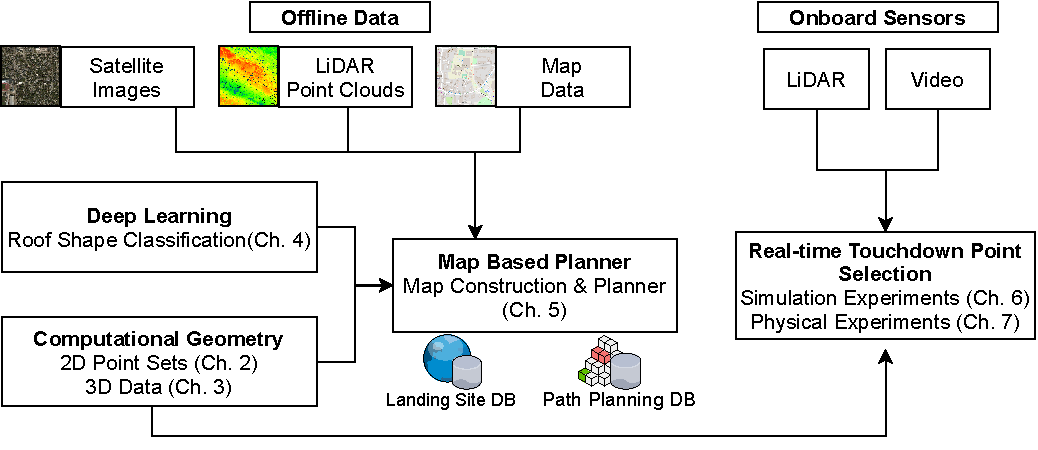
\includegraphics[width=0.70\linewidth]{chapter_1_intro/imgs/Challenge_Overview-thesis_overview.pdf}
    \caption{Overview of dissertation topics and structure.}
    \label{fig:ch1_thesis_overview}
\end{figure}

% \emph{How to efficiently construct databases from publicly available data to identify minimal-risk landing site for sUAS.}. Our previous stated observation of flat rooftop motivates 

% Numerous public datasets exist to aid construction of maps for aircraft urgent landing including satellite images, airborne LiDAR point clouds, census data, and existing building outlines. Our first goal is to efficiently transform this raw data into a risk evaluated landing site database which may be used for landing site selection and path planning.  Previous research has used such data to identity terrain based landing but none to our knowledge has focused on extracting flat rooftops \cite{atkins_emergency_2006, meuleau_emergency_2009, sankararaman_towards_2017, di_donato_evaluating_2017}. Our second goal is the construction of an efficient multi-goal planner which will account for both the intrinsic landing site risk as well as path risk. 



% Talk about data. Talk about the forms of data we have available for us to use: satellite images, airborne lidar points clouds, building outlines, census data. A host of information to help us make decision about places we can land.


\paragraph{Polygons from 2D Point Sets}

Characterizing the shape of a set of 2D points $\mathcal{P}$ has been a long-term focus of computational geometry research. A convex hull is defined as the smallest convex polygon that fully encapsulates all points in a set $\mathcal{P}$ as shown in Figure \ref{fig:ch1_convex_concave_1}.  Although widely used to estimate shape, point sets with non-convex distributions are poorly characterized by a convex hull \cite{duckham_efficient_2008}.  Convex hull over-estimation can be a serious issue when the points represent physical objects, e.g., obstacle free navigable areas. Several algorithms have been developed to construct shapes that ``fit'' or ``cover'' point sets more closely. These shapes are often termed non-convex polygons or concave hulls. 

The most notable examples of these algorithms are $\alpha$-shape \cite{edelsbrunner_shape_1983}, Spatialite concave hull \cite{furieri_spatialite_2017}, and PostGIS concave hull \cite{open_source_geospatial_foundation_postgis_2019}. Each is widely used in the computational geometry and GIS communities. These methods can extract the exterior boundary of a point set and also interior holes.  However, many of these methods are extremely slow motivating this dissertation to create an efficient non-convex (multi)polygon extraction algorithm called Polylidar. A key insight of this work is a novel boundary following method that contrasts computationally-expensive geometric unions of triangles. Real-world and synthetic benchmarks are presented to comparatively evaluate Polylidar speed and accuracy. Results show comparable accuracy and more than four times speedup compared to other open source concave polygon extraction methods. An example polygon from Polylidar is shown in Figure \ref{fig:ch1_convex_concave_2}.

% This dissertation uses the Open GeoSpatial Consortium (OGC) standard \cite{herring_opengis_2006-1} for defining \textit{linear ring} and \textit{polygon}. A linear ring is a consecutive list of points that is both closed and simple. This requires a linear ring to have non-intersecting line segments that join to form a closed path. The key components of a valid polygon are a single exterior linear ring representing the \emph{shell} of the polygon and a set of linear rings (possibly empty) representing \emph{holes} inside the polygon. 


\begin{figure}[t]

  \begin{subfigure}[t]{.22\linewidth}
    \centering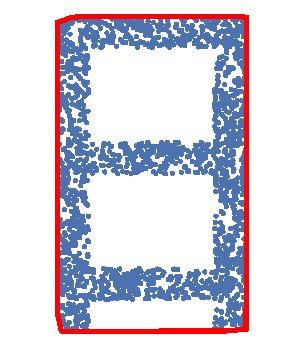
\includegraphics[width=.95\linewidth]{chapter_3_polylidar3d/imgs/concave_vs_convex_lettera_1.pdf}
    \caption{\label{fig:ch1_convex_concave_1}}
  \end{subfigure}
  \begin{subfigure}[t]{.22\linewidth}
    \centering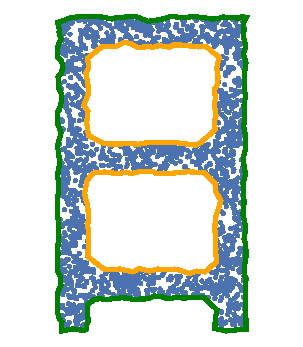
\includegraphics[width=.95\linewidth]{chapter_3_polylidar3d/imgs/concave_vs_convex_lettera_3.pdf}
    \caption{\label{fig:ch1_convex_concave_2}}
  \end{subfigure}
  \begin{subfigure}[t]{.26\linewidth}
    \centering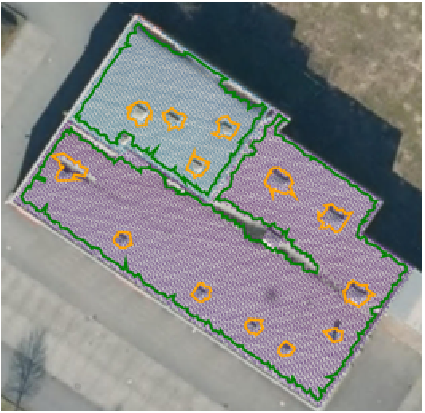
\includegraphics[width=.95\linewidth]{chapter_1_intro/imgs/rooftop_example_simple.pdf}
    \caption{\label{fig:ch1_rooftop_polygon}}
  \end{subfigure}
  \begin{subfigure}[t]{.26\linewidth}
    \centering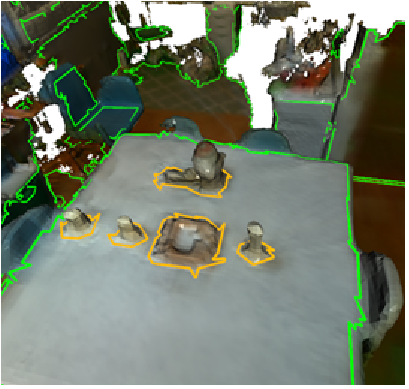
\includegraphics[width=.95\linewidth]{chapter_1_intro/imgs/mesh_example_simple.pdf}
    \caption{\label{fig:ch1_mesh_polygon}}
  \end{subfigure}
  \caption{(a,b) Examples of a convex hull (red) and a non-convex polygon with holes from a 2D point set. (c,d) Examples of Polylidar3D's non-convex multi-polygon extraction from airborne LiDAR point clouds (colored by height) and a user provided mesh, respectively}\label{fig:ch1_polygon_examples}
\end{figure}


\paragraph{Polygons from 3D Data}

Flat surfaces are pervasive in engineered structures and also occur in natural terrain. For example, structures such as walls, floors, rooftops, and roadways are often flat or ``flat-like". 
% Similarly, home and office furnishings are typically composed of multiple flat surfaces.
Sensors such as LiDAR and RGBD cameras generate dense 3D point clouds of these predominately flat surface environments. This observation has been exploited for tasks in localization and mapping \cite{pathak_online_2010},  digital preservation with Photogrammetry and laser scanning \cite{malihi_3d_2016, lerma_terrestrial_2010, balsa-barreiro_generation_2018}, and point cloud registration \cite{rusinkiewicz_efficient_2001}. Planar segmentation techniques are often used to group points belonging to a common flat surface \cite{feng_fast_2014, pham_geometrically_2016-1, schaefer_maximum_2019}. However points clouds are dense incurring high computational cost when used directly in higher level tasks. Planar point clouds can be converted to lower dimensional representations such as polygons.
% Polygons reduce map size, accelerate matching for localization \cite{lee_indoor_2012-1}, and support model reconstruction and object detection \cite{cao_roof_2017}. 

Prior work has investigated transforming planar points clouds to convex polygons \cite{biswas_planar_2012,poppinga_fast_2008}.  Non-convex polygons can be generated using techniques such as $\alpha$-shapes but operate strictly on 2D data, requiring the projection of each 3D planar point cloud and expensive triangulation \cite{lee_fast_2013, edelsbrunner_shape_1983}. Pixel-level boundary following of organized point clouds (e.g., range images) can be used to extract non-convex polygons but often only captures the exterior shell of the polygon \cite{lee_indoor_2012-1}. These methods do not capture interior holes in a polygon needed to capture obstacles on flat surfaces. 

% Finally, many of the proposed solutions are limited in their use of 3D data, only working on range images and unable to handle unorganized forms of 3D data.

This dissertation introduces Polylidar3D, a non-convex polygon extraction algorithm that takes as input either unorganized 3D point clouds (e.g., airborne LiDAR point clouds), organized point clouds (e.g., range images), or user-provided meshes. A core idea of this work is to transform all data inputs into a half-edge triangular mesh for which planar segmentation and polygon extraction may occur in parallel. Dominant plane normals are identified and used to parallelize and regularize planar segments in the mesh. Triangles having similar normals to a dominant plane are grouped. Each group (in parallel) then performs region growing accounting for normal orientation, Euclidean distance, and point to plane distance. Immediately after a plane has been segmented a polygon extraction task is dynamically spawned. The result is a general and extremely fast framework for non-convex polygon extraction of 3D data. Polylidar3D is used in this dissertation to extract polygonal representations of flat rooftop surfaces and generated meshes as shown in Figure \ref{fig:ch1_polygon_examples}c,d.


% Speed is an important consideration for many of the applications mentioned previously. Parallel algorithms written for multi-core CPUs and GPUs should be used to reduce latency. 



\paragraph{Roof Shape Classification}



% Satellite images and 3D point cloud data from airborne LiDAR sensors provide complementary data on buildings. High resolution satellite images offer rich information content and are generally available worldwide.  However, extracting 3D building information from 2D images is difficult due to occlusion, poor contrast, shadows, and skewed image perspectives \cite{zhou_seamless_2014}. LiDAR point clouds provide depth and intensity measurements that capture the features of roof shapes, yet LiDAR does not offer other world feature information from ambient lighting intensity and color. LiDAR point cloud data are often processed and converted to digital surface models (DSM) representing the top surface layer of any terrain.

In an effort to identify suitable flat-like rooftops for urgent landing, our approach is to first predict the roof shapes of all buildings in cities by fusing satellite and LiDAR data with machine learning techniques. % Such classification will allow identification of rooftops suitable for landing, but also be generally beneficial for the \ac{GIS} community. % solar power panel placement, localization for UAS, 
Classical machine learning algorithms such as support vector machines (SVM), logistic regression, and decision trees are often used in these classification scenarios but invariably face computational complexity challenges caused by the high dimensionality found in GIS data sources.   To employ these algorithms, a reduction in dimensionality through feature selection is often performed. Prior work has performed roof classification through Support Vector Machine (SVM) and Random Forest classifiers by reducing a digital surface model (DSM) image of a roof to a set of handcrafted features \cite{mohajeri_city-scale_2018, assouline_building_2017}. Recent work has used Convolutional Neural Networks (CNN) to process satellite images and/or building DSMs to predict roof shape \cite{partovi_roof_2017, alidoost_knowledge_2016}.

This dissertation processes satellite images, airborne LiDAR point clouds, and city map  building outlines to generate both a LiDAR image and a cropped satellite image of each building. CNNs are independently trained for each modality to extract high level features for roof shape prediction. Features from both images are then fused to train a random forest classifier. This research contributes the first large multi-city annotated dataset of over 4,500 rooftops to train, validate, and test models.  Example annotated rooftops are shown in Figure \ref{fig:ch1_rooftop_shape_examples}. Several CNN models and classical machine learning algorithms are evaluated.

\begin{figure}[t]
\centering
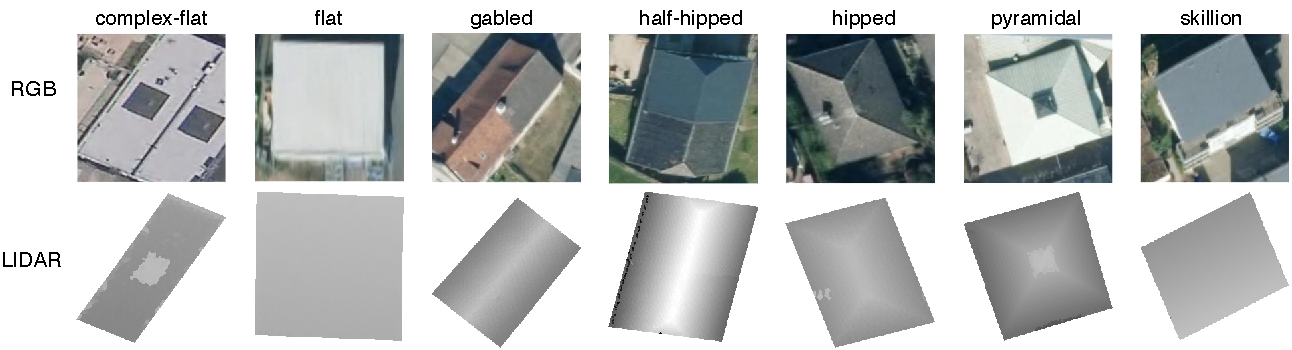
\includegraphics[width=0.99\textwidth]{chapter_4_roofshape/imgs/RoofShapes.pdf}
\caption{Satellite (RGB) and LiDAR example images of roof shapes.}
\label{fig:ch1_rooftop_shape_examples}
\end{figure}


\paragraph{Map based Planner}


% Urban areas typically do not offer classic emergency landing sites such as unpopulated open fields. This requires a planner to consider unconventional yet safe alternatives.

% We propose flat building rooftops as viable urgent landing sites for small UAS. During landing site selection, a map-based planner must be able to assess \emph{landing site risk} posed to the aircraft and bystanders at touchdown. The UAS may pose risk to people and property it overflies enroute, so the planner must also assess \emph{path risk} once the landing flight plan is known.  Landing site and path risk together offer an estimate of \emph{total risk}.

Map data used for urgent landing planning must have high integrity and low-latency access to support timely decision making. This dissertation proposes an offline data processing pipeline and online multi-objective, multi-goal landing planner that enable a UAS to minimize total risk when a nearby landing is required. Landing site and local area map information is pre-processed and stored onboard.  Roof shape classifiers and Polylidar3D are both used to identify flat-like rooftops and extract landing surfaces as polygons. Geometric algorithms are used to process flat rooftop polygons to find the largest inscribed circle that maximizes distance to obstacles and defines optimal touchdown location on each flat roof.  A multi-goal real-time landing planner explores available ground and rooftop landing sites likely to minimize overall total risk while greedily pruning options known to have higher risk.  Pareto fronts over landing site and path risk are generated for three urban regions: Witten, Germany; Ann Arbor, Michigan; and mid-town Manhattan in New York City. We statistically analyze results with respect to availability and quality of landing sites as well as execution time of the map-based planner.

\paragraph{Landing Site Identification and Selection Experiments (In Progress and Proposed)}

A small UAS should utilize available sensors to verify a safe touchdown point upon approach to a landing site. We build upon our previous methods for offline landing site identification and selection to  use on-board sensors generating point clouds in real-time. Prior work has investigated converting these point clouds to 2D disparity grids \cite{desaraju_vision-based_2015} or probabilistic elevation maps \cite{forster_continuous_2015}. These methods then apply computer vision kernels over the grids to smooth and identify ``flat'' touchdown points. 
% Sensors such as LiDAR, RGBD cameras, or monocular cameras utilizing Structure from Motion (SfM) can generate 3D point clouds of the landing site. 
An alternative to operating over a discretized image space is modelling the 3D mesh of the roof. Polylidar3D can be used to rapidly construct a surface mesh and extract polygonal representations of all flat surfaces while accounting for obstacles. Afterward the largest inscribed circle in each polygon is defined. For the final dissertation,  flight experiments with small multicopter UAS carrying LiDAR sensors will be conducted to demonstrate and evaluate real-time map generation for landing site safety validation (in areas with small UAS landing site maps) or real-time landing identification and selection (in areas without small UAS landing site maps). Tests will be conducted in the M-Air netted flight facility where motion capture can provide ground truth data to be compared with UAS-generated landing site maps and decisions. 


\paragraph{Contributions and Innovations \\}
% \vspace{1.5cm}
Specific contributions of this dissertation include: % things that have taken time / effort

\begin{itemize}[noitemsep]
  \item A faster open source library for non-convex (multi)polygon extraction from 2D point sets. An open source benchmark comparison of leading non-convex polygon extraction techniques in terms of accuracy and speed is provided. %\cite{Castagno_Github_Polylidar}.
%   \item An open source benchmark comparison of leading concave polygon extraction techniques from 2D point sets in terms of accuracy and speed.
  \item An efficient and versatile open source framework, Polylidar3D,  for non-convex (multi)polygon extraction from 3D data representing flat surfaces. Polylidar3D can handle unorganized and organized 3D point clouds as well as triangular meshes. Computation time is minimized with CPU multi-threading and GPU acceleration. %\cite{Castagno_Github_Polylidar}
  \item Multiple open source and reproducible experiments showing qualitative and quantitative benchmark results of Polylidar3D applied to sensors including LiDAR and RGBD cameras.
  \item A fast open source dominant plane normal estimation library, FastGA,  using a novel Gaussian Accumulator with efficient search.
  \item A deep learning framework for predicting roof shapes from a fusion of satellite image, airborne LiDAR point cloud, and existing building outline data. Over 4,500 buildings rooftops spanning three cities have been manually classified  for training, validation, and testing.
  \item A multi-goal planner that guarantees a risk-optimal solution is found rapidly by avoiding exploration of high-risk options. Plans are optimized over a combination of landing site and path risk metrics.
  \item (Proposed) Experimental UAS results of real-time landing site validation or identification/selection with Polylidar3D.
\end{itemize}
 
Specific innovations of this dissertation are: % things that have taken time / effort

\begin{itemize}[noitemsep]
      \item A novel computationally-efficient algorithm to extract non-convex polygons from 2D point sets while accounting for holes. The proposed method utilizes half-edge boundary following with edge-case detection instead of alternatives such as the expensive union of triangles.
      \item The first parallelized non-convex polygon extraction framework working with several forms of 3D data. Polygons represent dominant planar surfaces with interior holes representing the shape of obstacles embedded on their surface. Polylidar3D's speed and data input versatility allow its use for many applications.
    %   Triangle primitives are grouped according to dominant plane normals for which region growing occurs in parallel. Polygon extraction of segmented planar regions are spawned as dynamic tasks in a thread-pool. 
      \item The first large-scale multi-city analysis for predicting roof shapes. The provided annotated dataset contains diverse examples from small to large metropolitan city centers. 
      \item The first rigorous method to incorporate flat rooftops as candidate landing sites for urgent landing of small UAS in cities.  Optimal touchdown sites on rooftop surface are determined using geometric methods with risk evaluated according to size and proximity to alternative touchdown sites.
\end{itemize}


% Open Source C++ libraries (with Python bindings) are released at the following links:

% \begin{itemize}
%     \item Contribution 1 - {\small{ \url{https://github.com/JeremyBYU/polylidar/tree/polylidar2d}}}
%     \item Contribution 2 - {\small{ \url{https://github.com/JeremyBYU/polylidar}}}
%     \item Contribution 3 - {\small{\url{https://github.com/JeremyBYU/FastGaussianAccumulator}}}
%     \item Contribution 7 - TBD
% \end{itemize}

% Open Data sets are released at the following links:

% \begin{itemize}
%     \item Classified Roof Shape - {\small \url{https://www.mdpi.com/1424-8220/18/11/3960/s1}}
% \end{itemize}


\paragraph{Products}
Publications, software, and datasets connected to this dissertation are:
\vspace{0.2cm}

\textbf{Conference}
\vspace{0.20cm}
\begin{itemize}[noitemsep]
    \item J. Castagno, C. Ochoa, and E. Atkins, ``Comprehensive Risk-based Planning for Small Unmanned Aircraft System Rooftop Landing,” in 2018 \emph{International Conference on Unmanned Aircraft Systems} (ICUAS), Jun. 2018, pp. 1031–1040, doi: 10.1109/ICUAS.2018.8453483.
    \item K. McDonough, J. Castagno, and J. Player, ``RANGR: Risk Aware Navigation and Gudiance Resilience,” presented at the \emph{AUVSI Xponential}, Denver, CO, USA, May 2018.
	\item J. Castagno and E. M. Atkins, ``Automatic Classification of Roof Shapes for Multicopter Emergency Landing Site Selection,” in 2018 \emph{Aviation Technology, Integration, and Operations Conference, American Institute of Aeronautics and Astronautics}, 2018.
\end{itemize}

\vspace{0.25cm}

\textbf{Journal}

\vspace{0.20cm}
\begin{itemize}[noitemsep]
    \item J. Castagno, M. Romano, P. Kuevor, and E. Atkins, ``Multi-UAV Wildire Boundary Estimation using a Semantic Segmentation Neural Network,” \emph{Journal of Aerospace Information Systems}. Sumbitted under review.
    \item J. Castagno and E. Atkins, ``Map-Based Planning for Small Unmanned Aircraft Rooftop Landing (In Press),” in \emph{Handbook on Reinforcement Learning and Control}, Springer, 2021. In Press.
    \item J. Castagno and E. Atkins, “Polylidar3D - Fast Polygon Extraction from 3D Data,” \emph{Sensors}, vol. 20, no. 17, Art. no. 17, Jan. 2020, doi: 10.3390/s20174819.
    \item J. Castagno and E. Atkins, “Polylidar - Polygons From Triangular Meshes,” \emph{IEEE Robotics and Automation Letters}, vol. 5, no. 3, pp. 4634–4641, Jul. 2020, doi: 10.1109/LRA.2020.3002212.
    \item J. Castagno and E. Atkins, “Roof Shape Classification from LiDAR and Satellite Image Data Fusion Using Supervised Learning,” \emph{Sensors}, vol. 18, no. 11, Art. no. 11, Nov. 2018, doi: 10.3390/s18113960.
\end{itemize}

\textbf{Open Source C++ libraries (with Python bindings)}

\begin{itemize}[noitemsep]
    \item J. Castagno, ``Polylidar3D,''   [Online]  Available: \url{https://github.com/JeremyBYU/polylidar}, 2020.
    \item J. Castagno, ``Fast Gaussian Accumulator,''   [Online]  Available: \url{https://github.com/JeremyBYU/FastGaussianAccumulator}, 2020.
    \item J. Castagno, ``Organized Point Filters,''   [Online]  Available: \url{https://github.com/JeremyBYU/OrganizedPointFilters}, 2020.
\end{itemize}

\textbf{Open Data Sets}

\begin{itemize}[noitemsep]
    \item J. Castagno, ``Annotated Roof Shape Dataset,''   [Online]  Available: \url{https://www.mdpi.com/1424-8220/18/11/3960/s1}, 2018.
\end{itemize}


 
\chapter{Polygons from 2D Point Sets}
 \label{ch:polylidar}
 % \section{Introduction}

% Video and LiDAR data are widely used in robotics to provide rich information about the environment. LiDAR and RGBD cameras generate point clouds for localization and mapping \cite{pathak_online_2010}, 3D modelling \cite{malihi_3d_2016}, and scene classification for autonomous navigation \cite{himmelsbach_fast_2010}. Flat surfaces such as walls and floors are key environmental elements to identify; they are often extracted using planar segmentation techniques \cite{feng_fast_2014, pham_geometrically_2016-1, schaefer_maximum_2019}.   However points clouds are dense incurring a high computational cost when used directly. A common simplifying approach transforms point clouds into lower dimensional representations such as lines and planes \cite{biswas_planar_2012}. Furthermore, polygonal representations of planes reduces map size and may accelerate matching for localization \cite{lee_indoor_2012-1}.

% Convex polygon representations of planar segments were proposed by \cite{biswas_planar_2012}. Convex polygons are simple and efficient to generate but ignore boundary concavities and overestimate area of the enclosed point set. Non-convex polygon representations may be generated using techniques such as boundary following outlined in \cite{lee_indoor_2012-1} or $\alpha$-shapes as proposed in \cite{lee_fast_2013}. However few methods also capture the interior holes within non-convex polygons. Safe robot navigation demands accurate capture of non-convex polygons with interior holes in real-time, requiring both speed and robustness.    

This abbreviated chapter summarizes Polylidar, an efficient algorithm to transform 2D point sets into simplified non-convex (i.e. concave) polygons with holes. Polylidar begins by triangulating the point set and filtering triangles given user-specified parameters such as maximum triangle edge length. Once filtering is complete, edge-connected triangles are combined into regions creating a set of triangular meshes representing the shape of the point set. Next, Polylidar converts each mesh region to a polygon through a novel boundary following method which accounts for holes. Figure \ref{fig:ch1_convex_concave}b shows Polylidar applied to a 2D point set while (c) shows Polylidar used on a plane segmented point cloud from an RGBD image.


\begin{figure}[ht] 
    \centering
  \subfloat[]{%
    \centering
       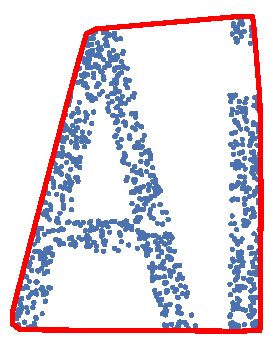
\includegraphics[clip, trim=0.0cm 0.1cm 0.0cm 0.25cm, width=0.20\linewidth]{chapter_2_polylidar/imgs/concave_vs_convex_0.pdf}
    }
    \label{fig:ch1_convex}\hfill
  \subfloat[]{%
  \centering
        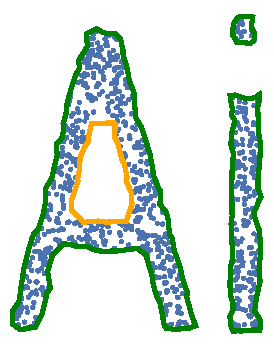
\includegraphics[clip, trim=0.0cm 0.1cm 0.0cm 0.25cm, width=.2\linewidth]{chapter_2_polylidar/imgs/concave_vs_convex_2.pdf}}
    \label{fig:ch1_concave} \hfill
  \subfloat[]{%
    \centering
      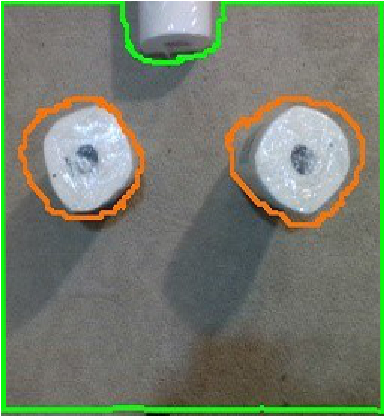
\includegraphics[width=0.25\linewidth]{chapter_2_polylidar/imgs/RealSensePictures-cropped_aspect.pdf}
    }
    \label{fig:ch1_realsense}\hfill\\
  \caption{(a) Convex hull of a point set (red); (b) MultiPolygon extraction using Polylidar (green).
  (c) Polygon extraction from a plane segmented point cloud from an Intel RealSense RGBD camera capturing paper towel rolls on a basement floor. 
  Note that Polylidar also identifies holes (orange).}
  \label{fig:ch1_convex_concave} 
\end{figure}

We show that Polylidar is approximately four times faster than leading open source approaches for concave polygon extraction. Polylidar's speed is attributed to rapidly identifying boundary edges (shell and holes) and then performing  boundary following to ensure a valid polygon is returned. 

\paragraph{Results}
% \section{Experiments}

Polylidar is benchmarked against other common concave hull extraction methods which also extract holes; all code is open source\footnote{https://github.com/JeremyBYU/concavehull-evaluation}. Three other implementations are tested: CGAL's Alpha Shape function and the ST\_ConcaveHull function from PostGIS and Spatialite. For uniformity, Polylidar and CGAL are set to use the same $\alpha$ parameter to guarantee exact shape reproduction. 
Three separate tests sets are created to evaluate the speed and accuracy of each method: plane segmented point clouds produced by an RGBD camera,  synthetic point sets from the state shapes of California (CA) and Hawaii (HI), and synthetic point sets generated form the English alphabet. All tests have a ground truth (multi)polygon, $GT$, to evaluate shape accuracy. Each implementation takes as input a point set and produces a concave shape, $CS$, which is similar to the ground truth polygon.  The $L^2$ error norm, the area of the symmetric difference between $GT$ and $CS$, is computed to enable evaluation of shape error $\frac{area((GT-CS) \cup (CS-GT))}{area(CS)}$. For brevity only the results of the alphabet shapes are shown in this summary. 



% \subsection{Alphabet Shapes}\label{sec:alphabet_shapes}

% {\color{blue}
Polygons from 26 capital letters of the English alphabet were generated and 2000 points randomly sampled inside.
%Some polygon letters naturally have holes such as ``A'', however no capital letters are MultiPolygons. Each letter was uniformly sampled to generate a 2000 point set and run through each algorithm. 
The ``A'' in Figure \ref{fig:ch1_convex_concave}b shows an example capital letter with the output of Polylidar's concave hull. Table \ref{table:alphabet_tests} provides aggregate statistics of all 26 test cases. Polylidar is about four times faster than the second fastest algorithm CGAL. Spatialite has marginally higher accuracy then both CGAL and Polylidar. 
% The alphabet shapes are significantly more concave than previous benchmarks. Documentation of PostGIS indicates that the run time grows quadratically as concavity increases leading to the high execution times observed \cite{open_source_geospatial_foundation_postgis_2019}.

%However PostGIS shape error and time are significantly higher than previously seen. This is because the alphabet shapes are significantly more concave then the tested state shapes, requiring a much smaller \emph{target percent} parameter for PostGIS (on average 0.38). Documentation of PostGIS indicates that the run time grows quadratically when reducing this parameter and at ``small'' values may fail to produce a concave shape \cite{postgis}.  PostGIS failed to produce any shape for the letters ``J'', ``L'', and ``M''. All other algorithms provided valid results for all test cases.
%  (reduced to 1000 points for visual clarity)

%  Polylidar continues to lead in speed, about 4.5 times faster than the next leading algorithm CGAL (shape error remains the same because of same $\alpha$ used). Spatialite continues to lead in accuracy by a marginal amount for the same reasons discussed previously. However PostGIS shape error and time are significantly higher than previously seen. This is because the alphabet shapes are significantly more concave then the tested state shapes, requiring a much smaller \emph{target percent} parameter for PostGIS (on average 0.38). 
% Documentation of PostGIS indicates that the run time grows quadratically when reducing this parameter and at ``small'' values may fail to produce a concave shape \cite{postgis}.  PostGIS failed to produce any shape for the letters ``J'', ``L'', and ``M''. All other algorithms provided valid results for all test cases.
% }
 
\begin{table}[!ht]
\centering
\caption{Alphabet Letter Results, 26 Shapes}
\label{table:alphabet_tests}
\begin{tabular}{lcccccc}
\toprule
{} & \multicolumn{3}{c}{$L^2$ error \%} & \multicolumn{3}{c}{Time (ms)} \\
{Algorithm} &    mean & std &  max &      mean &     std &     max \\
% Algorithm        &         &     &      &           &         &         \\
\midrule
% polylidar  &    12.8 & 1.8 & 16.8 &       1.8 &     0.3 &     2.9 \\
% cgal       &    12.8 & 1.8 & 16.8 &       6.8 &     0.8 &     9.8 \\
% postgis    &    36.5 & 9.9 & 53.7 &   18973.3 & 10786.2 & 39587.8 \\
% spatialite &    11.2 & 4.5 & 22.1 &     330.4 &    33.8 &   438.1 \\
Polylidar  &           12.8 & \textbf{1.8} & \textbf{16.8} &       \textbf{1.2} &    \textbf{0.3} &     \textbf{2.4} \\
CGAL       &           12.8 & \textbf{1.8} & \textbf{16.8} &       5.4 &    0.9 &     7.2 \\
PostGIS    &           36.5 & 9.9 & 53.7 &   13091.8 & 7500.6 & 28451.0 \\
Spatialite &           \textbf{11.2} & 4.5 & 22.1 &     230.2 &    6.3 &   242.9 \\
\bottomrule
\end{tabular}
\end{table}


\paragraph{Conclusion}
This chapter introduces Polylidar, an efficient 2D concave hull extraction algorithm that produces (multi)polygon output with holes. Comparison benchmarks of numerous test sets, similarly done in \cite{duckham_efficient_2008}, show Polylidar is faster than competing approaches with comparable or better accuracy. A full description of the algorithm with additional results is available in \cite{castagno_polylidar_2020}.


% Contributions of this chapter are:
% \begin{itemize}
%   \item A faster open source \cite{Castagno_Github_Polylidar} concave (multi)polygon extraction algorithm from 2D point sets.
%   \item A benchmark comparison of leading concave polygon extraction techniques in terms of accuracy and speed.
% \end{itemize}


% Below, Sections \ref{sec:background} and \ref{sec:prelim} provide background on non-convex shape generation and mathematical preliminaries, respectively. Section \ref{sec:methods} describes Polylidar algorithms, while Section \ref{sec:results} shows benchmark test results of Polylidar versus other methods.  Section \ref{sec:random_polygons_test} describes test results. Sections  \ref{sec:discussion} and \ref{sec:conclusion} provide discussion and conclusions.



% \section{Background}\label{sec:background}

% Characterizing the shape of a set of 2D points $\mathcal{P}$ has been a long-term focus of computational geometry research. A convex hull is defined as the smallest convex polygon that fully encapsulates all points in a set $\mathcal{P}$.  Although widely used to estimate shape, point sets with non-convex distributions are poorly characterized by a convex hull \cite{duckham_efficient_2008}.  Convex hull over-estimation can be a serious issue when the points represent physical objects, e.g., obstacle free navigable areas. Several algorithms have been developed to construct shapes that ``fit'' or ``cover'' point sets more closely. 

% Figure \ref{fig:ch1_convex_concave} compares convex and concave hulls. Figure \ref{fig:ch1_convex_concave}b is the multipolygon output of Polylidar described below.
% %One may argue that the red convex hull does not conform well to the point distribution but the green concave hull captures the shape of the letters more precisely. 
% While there is a unique convex hull, there is no true or unique concave hull.  Concave hull algorithm implementations can also have different output types.  Some return only an unordered set of edges while others return a single polygon.  Some algorithms return multiple disconnected polygons (multipolygon), and some can generate holes inside a polygon.

% The $\alpha$-shape algorithm is an early strategy to generate a family of shapes ranging from a convex hull to a point set  \cite{edelsbrunner_shape_1983}. The parameter $\alpha$ dictates the radius of a closed disk used to prune/remove area in the convex hull. This disk is allowed to move freely shaving off the excess shape until it finds points. When disk radius is large, ideally infinite, the convex hull is produced; when disk radius is infinitesimally small only the points remain. A common implementation of $\alpha$-shape organizes points using Delaunay triangulation and filters triangles whose circumcircle radius is less than $\alpha$.  The final shape is represented by the remaining edges and triangles.  Note that the $\alpha$-shape method creates multiple non-intersecting shapes with the possibility of holes. 

% % The algorithm in \cite{Duckham2008} produces polygons from point sets called $\chi$-shapes. Like some $\alpha$-shape implementations, the $\chi$-shape approach begins with Delaunay triangulation to order and spatially connect data points.  The algorithm differs by iteratively removing the longest exterior edges from triangulation based on a specified maximum length parameter $l$. A corner case occurs  when edge removal results in a non-simple polygon, i.e., the polygon wraps into itself; in this case edge removal is skipped.  The $\chi$-shape produced is a single polygon with no possibility of holes.

% The geospatial software library Spatialite \cite{furieri_spatialite_2017}, an extension to SQLite \cite{hipp_sqlite_2020}, contains a concave hull extraction procedure. The algorithm again starts with Delaunay triangulation then analyzes the distribution of each triangle's edge length to determine mean $\mu_l$ and standard deviation $\sigma_l$. Any triangle with edge length greater than $C \cdot \sigma_l  + \mu_l$ is removed, where $C$ is a user-defined parameter. The final geometry returned is the union of all triangles computed with GEOS, a high performance open source geometry engine. The output may be a multipolygon (i.e., multiple disjoint polygons) with the possibility of holes inside each. 

% PostGIS is a geospatial database of computational geometry routines such as the concave hull method in \cite{open_source_geospatial_foundation_postgis_2019}. This algorithm first calculates the convex hull and then shrinks the hull by adjusting vertex connections to closer points which ``cave in'' the hull.  This process recursively shrinks a boundary until a user-specified percent reduction in area from the convex hull is achieved. The resulting shape is a single polygon with the possibility of holes. 

% \begin{table}[ht]
% \centering
% \caption{Concave Hull Extraction Methods}
% \label{table:compare_alg}
% \begin{tabular}{ccc}
% \hline
% Algorithm                                                   & Output                                                           & Holes? \\ \hline
% \begin{tabular}[c]{@{}c@{}}CGAL $\alpha$-shape\end{tabular}   & \begin{tabular}[c]{@{}c@{}}unordered\\ set of edges\end{tabular} & Yes    \\
% % $\chi$-shapes                                             & \begin{tabular}[c]{@{}c@{}}Unordered\\ Set of Edges\end{tabular} & No     \\
% Spatialite                                                 & (multi)polygon                                                   & Yes    \\
% PostGIS                                                       & polygon                                                          & Yes    \\
% Polylidar (new)                                                   & (multi)polygon                                                   & Yes    \\ \hline
% \end{tabular}
% \end{table}

% Table \ref{table:compare_alg} provides a summary  of the concave hull algorithms discussed above. The Computational Geometry Algorithms Library (CGAL) is  used as the implementation of the $\alpha$-shape method \cite{the_cgal_project_cgal_2019}. Note that the time complexity of all algorithm implementations, with the exception of PostGIS, is $\mathcal{O}(n\log{}n)$.  Our paper contributes a procedure to more rapidly compute (multi)polygon output with the possibility of holes.  Though this is a complex output to generate, we show through benchmarks that our algorithm and implementation outperforms other available approaches.

% \section{Preliminaries}\label{sec:prelim}

% A 2D \textit{point set} is an arbitrarily ordered set of two dimensional points in a Cartesian reference frame. Each point is defined by orthogonal bases $\hat{\mathbf{e}}_x$ and $\hat{\mathbf{e}}_y$  with
% \begin{equation}
% \label{eq:point}
%     \vec{{p}_{i}}=x\,\hat{\mathbf{e}}_x+y\, \hat{\mathbf{e}}_y= [x,y]
% \end{equation}
% where $x,y$ are plane coordinates.

% An $n$-point array $\mathcal{P} = \{ \vec{{p}_{1}}, \vec{{p}_{i}}, \ldots, \vec{{p}_{n}} \}$ contains points $\vec{{p}_{i}} \in \mathbb{R}^2$ indexed by $i$.  A triangular mesh $ \mathcal{T}$ is defined by
% \begin{equation}
% \label{eq:tri}
%     \mathcal{T} = \{ t_1, t_i, \ldots, t_{k} \}
% \end{equation}
% where each $t_i$ is a triangle with vertices defined by three point indices $\{i_1, i_2, i_3\} \in \left[1,n\right]$ referencing points in $\mathcal{P}$.

% We follow the Open Geospatial Consortium (OGC) standard \cite{herring_opengis_2006-1} for defining \textit{linear ring} and \textit{polygon}. A linear ring is a consecutive list of points that is both closed and simple. This requires a linear ring to have non-intersecting line segments that join to form a closed path. The key components of a valid polygon are a single exterior linear ring representing the \emph{shell} of the polygon and a set of linear rings (possibly empty) representing \emph{holes} inside the polygon. 
 
 
\chapter{Polygons from 3D Data}
 \label{ch:polylidar3d}
 % \section{Introduction}
% Flat surfaces are pervasive in engineered structures and also occur in natural terrain. For example, structures such as walls, floors, rooftops, and roadways are often flat or ``flat-like". Similarly, home and office furnishings are typically composed of multiple flat surfaces. Sensors such as LiDAR and RGBD cameras generate dense 3D point clouds of these predominately flat surface environments. This observation has been exploited for tasks in localization and mapping \cite{pathak_online_2010},  digital preservation with Photogrammetry and laser scanning \cite{malihi_3d_2016, lerma_terrestrial_2010, balsa-barreiro_generation_2018}, and point cloud registration \cite{rusinkiewicz_efficient_2001}. Planar segmentation techniques are often used to group points together belonging to a flat surface \cite{feng_fast_2014, pham_geometrically_2016-1, schaefer_maximum_2019}. However points clouds are dense incurring a high computational cost when used directly in higher level tasks. Planar point clouds can be converted to lower dimensional representations such as polygons. Polygons reduce map size, accelerate matching for localization \cite{lee_indoor_2012-1}, and support model reconstruction and object detection \cite{cao_roof_2017}. 

% Planar points clouds may be converted to convex polygons \cite{biswas_planar_2012}. Convex polygons are simple and efficient to generate but often do not represent the true shape of a point set. Non-convex polygons may be generated using techniques such as $\alpha$-shapes but operate strictly on 2D data, requiring the projection of each 3D planar point cloud and expensive triangulation \cite{lee_fast_2013, edelsbrunner_shape_1983}. Pixel-level boundary following of organized point clouds can be used to extract non-convex polygons but often only captures the exterior shell of the polygon \cite{lee_indoor_2012-1}. These methods are not able to capture \emph{interior} holes in a polygon representing the shape of obstacles on flat surfaces. Finally, speed is an important consideration for many of the applications mentioned previously. Parallel algorithms written for multi-core CPUs and GPUs should be used to reduce latency. 



This chapter summary presents Polylidar3D, a non-convex polygon extraction algorithm that takes as input either unorganized 3D point clouds (e.g., airborne LiDAR point clouds), organized point clouds (e.g., range images), or user-provided meshes. The non-convex polygons extracted represent flat surfaces in a 3D environment, while interior holes represent obstacles on these surfaces.  Figure \ref{fig:ch3_polylidar_overview} provides an overview of Polylidar3D's data input, front-end, back-end, and output. Currently only one planar direction can be extracted from unorganized 3D point clouds while all other 3D data inputs do not have this limitation. The front-end transforms input data into a half-edge triangular mesh.  This representation provides a common level of abstraction offering increased efficiency for back-end operations. The back-end is composed of four core algorithms: mesh smoothing, dominant plane normal estimation, planar segment extraction, and polygon extraction.  Polylidar3D outputs planar triangular segments, sets of flat connected triangles, and their polygonal representations. Polylidar3D is extremely fast, typically executing in a few milliseconds. It makes use of CPU multi-threading and GPU acceleration when available. 

% Main contribution of this chapter are:

% \begin{itemize}
%   \item An efficient and versatile open source \cite{Castagno_Github_Polylidar} framework for concave (multi)polygon extraction for 3D data. Input can be unorganized/organized 3D point clouds or user-provided meshes.
%   \item A fast open source \cite{Castagno_Github_fastga} dominant plane normal estimation procedure using a Gaussian Accumulator that can also be used as a stand-alone algorithm.
%   \item Multiple diverse open source experiments showing qualitative and quantitative benchmark results from data sources including LiDAR and RGBD cameras \cite{Castagno_Github_Polylidar3D_Kitti, Castagno_Github_Polylidar3D_RealSense, Castagno_Github_Polylidar_Synpeb}.
%   \item Improved half-edge triangulation efficiency for organized point clouds; CPU multi-threaded and GPU accelerated mesh smoothing \cite{Castagno_Github_opf}. 
%   \item Planar segmentation and polygon extraction performed in tandem using task-based parallelism to reduce latency for time-critical applications. 
% \end{itemize}

\begin{figure}[ht]
    \centering
    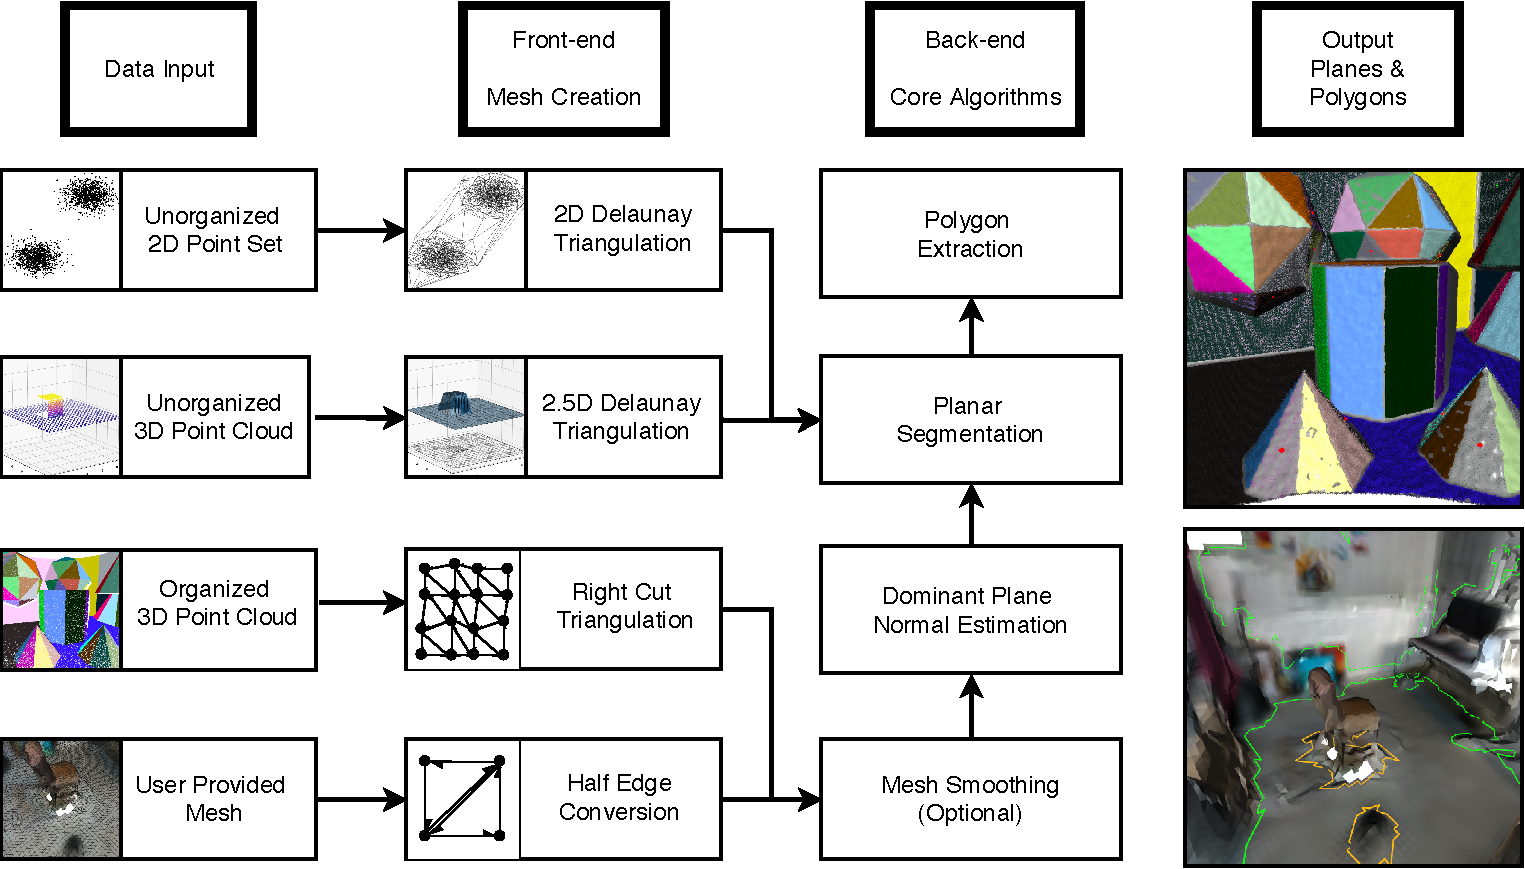
\includegraphics[width=.95\linewidth]{chapter_3_polylidar3d/imgs/Polylidar3DArchitecture-SimplifedV4.pdf}
    \caption{Overview of Polylidar3D. Input data can be 2D point sets, unorganized/organized 3D point clouds, or user-provided meshes. Polylidar3D's front-end transforms input data to a half-edge triangulation structure. The back-end is responsible for mesh smoothing, dominant plane normal estimation, planar segmentation, and polygon extraction. Polylidar3D outputs both planes (sets of spatially connected triangles) and corresponding polygonal representations. An example output of color-coded extracted planes from organized point clouds is shown (top right). An example of extracted polygons from a user-provided mesh is shown (bottom right). The green line represents the concave hull; orange lines show interior holes representing obstacles.} %Note that only one planar direction can be extracted for unorganized 3D point clouds. This is suitable for airborne LiDAR point clouds. }
    \label{fig:ch3_polylidar_overview}
\end{figure}


\paragraph{Framework Highlights}

A key part of Polyidar3D is estimating dominant plane normals within a 3D scene using a novel Gaussian Accumulator, FastGA. A Gaussian Accumulator discretizes the surface of the unit sphere (S2) into individual cells creating ``bins'' of a histogram. Plane normals from a scene are integrated in the accumulator where subsequent peak detection isolates dominant planes. Unlike other methods that partition the sphere in polar coordinates \cite{borrmann_3d_2011, limberger_real-time_2015}, FastGA tessellates the unit sphere with triangles by recursively subdividing the primary faces of an icosahedron. This removes issues with unequal weighting during accumulation, singularities at the poles, and non-equivariant kernels for peak detection.  Recursion level dictates the approximation of the unit sphere. The integration strategy does not rely upon K-D trees but instead uses a global spatial index from space-filling curves followed by local neighborhood search. All data structures are determined at compile time. We unfold the refined icosahedron into a 2D image in a particular way that guarantees equivariant kernels as outlined in \cite{cohen_gauge_2019} . Standard 2D image peak detection is then performed with nearby peaks clustered using agglomerative hierarchical clustering.



\paragraph{Results}

This section summary offers examples of Polylidar3D applied to real-world and synthetic 3D data. Our full paper (and dissertation chapter) shows examples of Polylidar3D applied to unorganized 3D points including airborne LiDAR point clouds and point clouds generated on a moving vehicle.  Additional experiments of organized point clouds including RGBD cameras as well as a challenging synthetic benchmark set are provided. A final analysis of Polylidar3D applied to 3D meshes explores how polygon extraction scales with additional CPU cores. For brevity only the comparison benchmark set is shown. 

% \subsection{SynPEB Benchmark}

Polylidar3D was evaluated on SynPEB, a benchmark dataset used to evaluate plane segmentation algorithms and created by the authors of PPE  \cite{schaefer_maximum_2019}. SynPEB is generated from a room populated with various polyhedra such that each image contains an average of 42.6 planes. LiDAR scans are simulated with different levels of normally-distributed radial and tangential noise producing organized point clouds of size 500 $\times$ 500. There are four levels of tangential noise in the dataset with 0.5 mdeg, 1 mdeg, 2 mdeg, and 4 mdeg standard deviation.  Data is partitioned into a training set to tune algorithm parameters and a test set for evaluation. The combination of high-noise data and numerous small, connected but distinct planes results in challenges for plane segmentation.% as shown in Figure \ref{fig:synpeb_pics}. 
%The noisy color-coded ground truth point cloud is shown in (a), a zoomed-in section of the generated mesh with no smoothing is shown in (b),  our Laplacian and bilateral smoothing is shown in (c), and (d) and (e) show the planes and polygons generated by Polylidar3D. 

Table~\ref{table:synpeb_results} shows benchmark test results (1mdeg of tangential noise) of Polylidar3D against other plane segmentation methods. The~results of other methods including timings are provided in Schaefer et al.~\cite{schaefer_maximum_2019}.  Note that execution times cannot be directly compared but will give an idea of real-time capability. Polylidar3D produces both a point set and polygonal representation of identified planes; however, this benchmark must be evaluated by the point set.   A~``plane'' is considered correctly identified if its point set overlaps with the ground truth plane with the standard 80\% threshold described in Hoover et al.~\cite{hoover_experimental_1996}. Key metrics are $f$ representing the percent of ground truth planes identified, $k$ indicating percent of the point cloud correctly identified, and~RMSE quantifying accuracy of each plane fit. Variables $n_o$, $n_u$, $n_m$, and~$n_s$ represent the absolute numbers of  oversegmented,  undersegmented,  missing,  and~spurious  planes, respectively,  compared  to  the  ground-truth  segmentation. See~\cite{schaefer_maximum_2019,hoover_experimental_1996} for detailed definitions of these metrics. %Red, green, and~yellow blocks in Figure~\ref{fig:synpeb_d} represent missed, spurious, and~oversegmented planes, respectively. 
An $f$ metric of 47.3\% indicates Polylidar3D did not capture most planes in the benchmark, but the $k$ metric of 78.3\% indicates Polylidar3D did well in capturing large dominant planes comprising most of the point cloud.  Additionally there are fewer spurious, over~segmented, and~under segmented planes generated by Polylidar3D than with other methods. Polylidar3D's RMSE value is also lowest, indicating predicted planes have a good fit. Plane segmentation is accomplished in less time, especially in comparison to PPE. Defined $f$ and $k$ metrics indicate PPE does an excellent job of capturing the numerous small planes in the scene but fails slightly more often in capturing large dominant planes.  Polylidar3D uniquely generates concave polygons providing a condensed representation of identified planes. Note polygon generation is included in Polylidar3D timing.





%  Note that RMSE is computed on input noisy point cloud (as all other implementations). 
\begin{table}[H]
\centering
\caption{SynPEB Benchmark~Results.  }
\label{table:synpeb_results}
\begin{tabular}{@{}ccccccccc@{}}
\toprule
\textbf{Method}                                  & $\textbf{f}$ {\textbf{[}}\textbf{\%}{\textbf{]}} & $\textbf{k}$ {\textbf{[}}\textbf{\%}{\textbf{]}} & \textbf{RMSE} {\textbf{[}}\textbf{mm}{\textbf{]}} & $\textbf{n}_\textbf{o}$ & $\textbf{n}_\textbf{u}$ & $\textbf{n}_\textbf{m}$ & $\textbf{n}_\textbf{s}$ & \textbf{time}\\ \midrule
PEAC~\cite{feng_fast_2014}              & 29.1         & 60.4         & 28.6          & 0.7   & 1.0   & 26.7  & 7.4   & \textbf{33 ms}\\
MSAC~\cite{torr_mlesac_2000}            & 7.3          & 35.6         & 34.3          & 0.3   & 1.0   & 36.3  & 10.9  & 1.1 s\\
PPE~\cite{schaefer_maximum_2019}      & \textbf{73.6}         & 77.9         & 14.5          & 1.5   & 1.1   & 7.1   & 16.5  & 1.6 hr\\
Polylidar3D (proposed)                  & 47.3         & \textbf{78.3}         & \textbf{7.2}           & \textbf{0.1}   & \textbf{0.3}   & \textbf{22.8}  & \textbf{4.9}  & 34 ms\\ \bottomrule
\end{tabular}
\end{table}


\paragraph{Conclusion}
This chapter introduced Polylidar3D, a non-convex polygon extraction framework for capturing flat surfaces from a variety of 3D data sources. Polylidar3D has been evaluated in five separate experiments with airborne LiDAR point clouds, automotive LiDAR point clouds, RGBD videos, synthetic LiDAR benchmark data, and meshes of indoor environments. Qualitative and quantitative results demonstrate Polylidar3D's speed and versatility. A complete description of the framework and individual algorithms with additional results is available in \cite{castagno_polylidar3d_2020}.


% Below, Sections \ref{sec:background} and \ref{sec:prelim} provide background and mathematical preliminaries, respectively. Section \ref{sec:methods_mesh_creation} describes Polylidar3D's front-end methods for mesh creation. Section \ref{sec:methods_mesh_smoothing} outlines optional mesh smoothing while Section \ref{sec:methods_fastga} introduces our dominant plane normal estimation algorithm. Section \ref{sec:methods_polylidar} describes plane and polygon extraction with parallelization techniques. Section \ref{sec:methods_polylidar_polygon_filtering} proposes optional post-processing methods to refine and simplify the polygons.  Section \ref{sec:results} provides qualitative results as well as quantitative benchmarks. Sections \ref{sec:discussion} and \ref{sec:conclusion} provide discussion and conclusion, respectively. 
 
 
\chapter{Roof Shape Classification from Satellite Images and LiDAR Data  }
 \label{ch:roofshape}
 % \section{Introduction}
% Geographic information system (GIS) data are openly available for a variety of applications. Data~on terrain height and type have historically been available, with high-accuracy labeled data now increasingly available, e.g., building footprints and heights.  Systematic characterization of building roof architecture and slope offers a new dimension to traditional terrain data.  These data could be used to rapidly identify building change or damage from the air, to improve in-flight localization capabilities in GPS-denied areas, and to inform small Unmanned Aircraft Systems (UAS) of alternative ditching sites, a problem previously investigated by the authors \cite{ochoa_fail-safe_2017, castagno_comprehensive_2018}.   Databases such as OpenStreetMap (OSM)~\cite{openstreetmap_contributors_planet_2017} provide limited roof information, but such data have been manually entered to-date thus is~sparse. 


This chapter summary describes research to fuse satellite imagery and airborne Light Detection and Ranging (LiDAR) data through multiple stages of machine learning classifiers to accurately characterize building rooftop shape.  With these results, roof geometries worldwide can be stored in an easily-accessible format for UAS, GIS, or other applications. Supervised training datasets are generated by combining building outlines, satellite, and LiDAR data. The resulting annotated dataset provides individual satellite image and LiDAR (depth) image representations for each building roof. Roof shapes are automatically categorized through a combination of convolutional neural networks (CNNs) and classical machine learning. Transfer learning is employed in which multiple pre-trained CNN model architectures and hyper-parameters are fine-tuned and tested. The best-performing CNN for both satellite and LiDAR data inputs is used to extract a reduced feature set which is then fed into either support vector machine (SVM) or random forest classifiers to provide a single roof geometry decision.  Validation and test set accuracies are evaluated over a suite of different classifier options to determine the best model(s). A range of urban environments are used to train and test the proposed models. Data from Witten, Germany; Ann Arbor, Michigan; and the Manhattan borough of New York City, New York are collected and manually labeled to represent small to large metropolitan city centers. We show that combining datasets from both small and large cities leads to a more generalized model and improves performance. Figure \ref{fig:outline_methods} provides an overview of the data processing pipeline and illustrates a {UAS localization and contingency landing} use case. %\cite{Castagno2018ICUAS}.

\begin{figure}[ht]
\centering
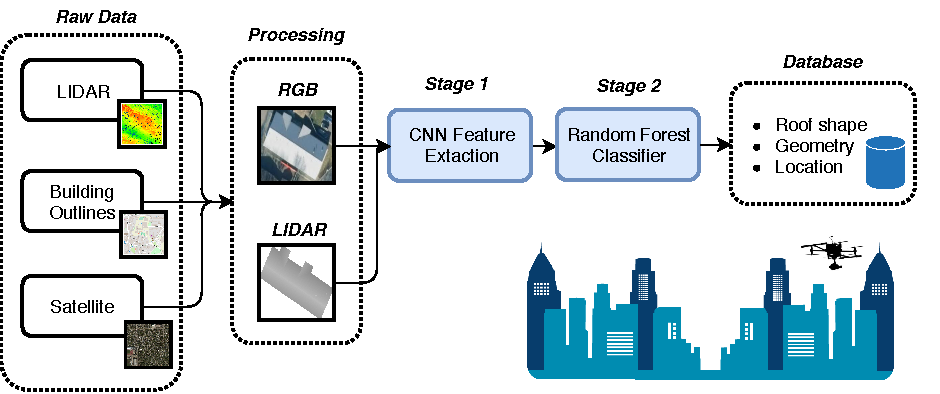
\includegraphics[width=0.70\textwidth]{chapter_4_roofshape/imgs/overview_process.pdf}
\caption{Roof classification data fusion and processing pipeline. LiDAR, building outlines, and satellite images are processed to construct RGB and LiDAR images of a building rooftop. In Stage    1, these images are fed into a CNN for feature extraction, while Stage    2 uses these features with a random forest for roof classification. These data can be stored for quick reference, e.g., navigation or emergency landing site~purposes. }
\label{fig:outline_methods}
\end{figure}




\paragraph{Results}

After training and validating a multitude of machine learning architectures, the best model is selected to be evaluated on two independent test sets. Test Set 1 comes from the 20\% withheld data representing the cities of Witten and New York City. The second test set from Ann Arbor is completely independent; the model was never trained on data from this region. The total accuracy for Test Set 1 is 87.2\%, while Test Set 2  scored 86.7\%. Confusion matrices for both test sets are shown in Figure  \ref{fig:ch1_dual_tes_cm}. The row-wise percentage of each cell is computed and color-coded along with the specific quantity classified in parentheses underneath. For both test sets one of the largest error sources is confusion between \texttt{complex-flat} and \texttt{flat} roofs.
For urgent landing use cases, both classes may be combined to a final ``flat-like'' class. To ensure only reliable predictions one can apply a confidence threshold for prediction. An 80\% confidence threshold results in a precision of 95\% with a recall of greater than 70\%. 


% The~authors found difficulty in labeling some flat-like roof examples, especially ones that bear traits of both classes; it is clear this confusion carried over into the trained model. In some cases, a roof is on the threshold of being \texttt{flat} or \texttt{complex-flat}, and this ambiguity makes it difficult to provide a consistent ``correct'' answer.  Indeed, this case often applies between the \texttt{complex-flat} and \texttt{unknown} labels as well:  When~does a~\texttt{complex-flat} roof become too complex to support a safe small UAS landing? The~authors attempted to be consistent in answering this question when labeling data, however edge cases were observed. 

% Table \ref{table:quality_metrics1} and \ref{table:quality_metrics2}  list  results for recall (completeness), precision (correctness), and~quality for Test Set     1 and Test Set     2, respectively. Note that there were no \texttt{pyramidal} roofs shapes in the Ann Arbor test set and too few \texttt{half-hipped} and \texttt{skillion} roofs to calculate valid metric~results.


\begin{figure}[ht]
    \centering
    \begin{subfigure}[t]{0.45\columnwidth}
        \centering
        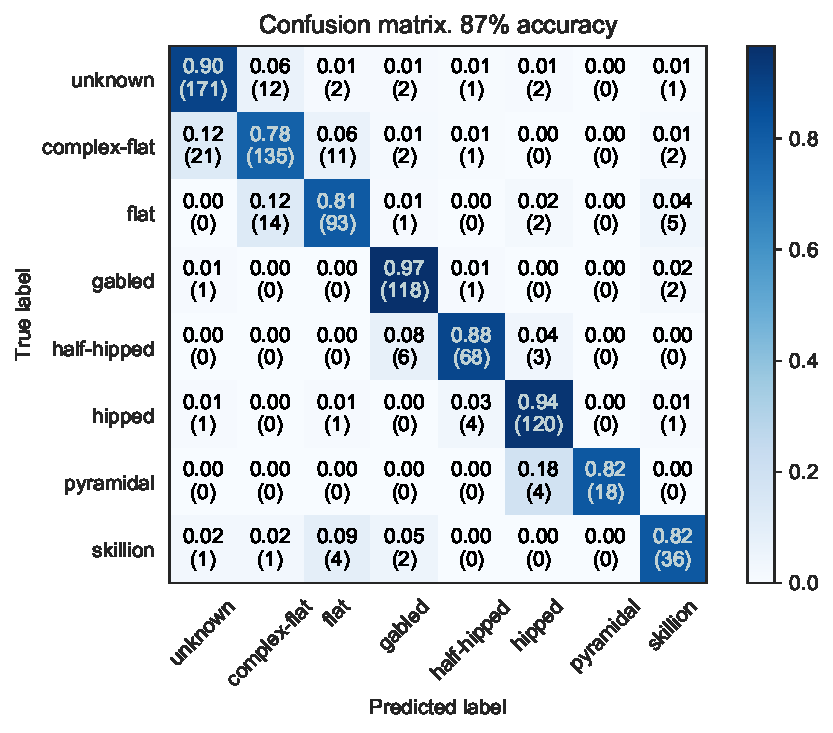
\includegraphics[width=0.90\textwidth]{chapter_4_roofshape/imgs/allclasses_combined_dual.pdf}
        \caption{Test Set     1}
        \label{fig:ch1_dual_test_combined_cm}
    \end{subfigure}
    \hfill
    \begin{subfigure}[t]{0.45\columnwidth}
        \centering
        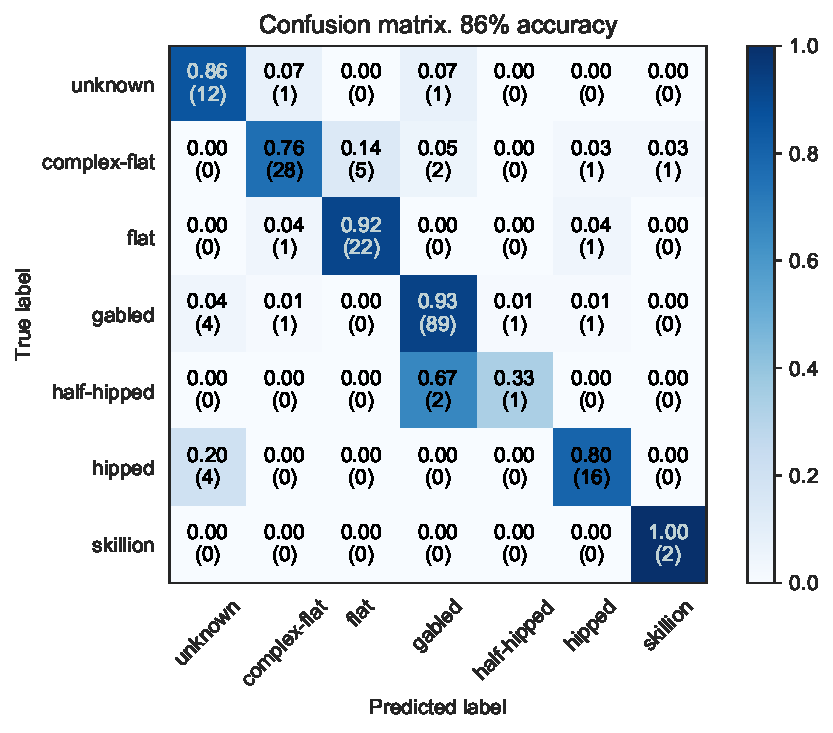
\includegraphics[width=0.90\textwidth]{chapter_4_roofshape/imgs/allclasses_aa_annarbor_dual.pdf}
        \caption{Test Set     2}
        \label{fig:ch1_dual_test_annarbor_cm}
    \end{subfigure}
    \vspace{-1pt}
    \caption{Confusion Matrices for Test Set 1 (Witten/Manhattan) and Test set 2 (Ann Arbor). }
    \label{fig:ch1_dual_tes_cm}
    \hfill
\end{figure}

\vspace{-1cm}
\paragraph{Conclusion}
Satellite images, LiDAR point clouds, and building outlines were processed to construct individual image representations of depth and color of roof shapes.  The final model uses deep learning for feature extraction and a random forest algorithm for subsequent roof shape classification. Generalized models and test datasets show promise for applying machine learning to automatically label roof shapes around the world with high confidence.
Full analysis of all models and results can be found in our paper \cite{castagno_roof_2018}.


% \begin{itemize}
%     \item Over 4500 building roofs spanning three cities have been manually classified and archived with a satellite and LiDAR depth image pair. This dataset is released with this paper.%NOTE: ?4500?
%     \item A ``complex-flat'' and ``unknown'' roof shape classe enable the machine classifier to distinguish flat roofs with infrastructure (e.g., air conditioning and water towers), unfamiliar roof shapes, and~images of poor quality.
%     % \item This paper significantly reduces the set of outliers that previously required manual removal for training and test datasets (from 45\% in \cite{Castagno2018} down to 5\% in this paper). This paper's test set accuracies represent a reasonable expectation of results when deployed in new areas.
%     \item An analysis of confidence thresholding is presented to improve the model's predictive power. This ensures only correct labels are assigned which is critical for use in high risk scenarios. 
%     \item Expanded results are presented from use of a single trained classifier (over Witten and Manhattan) tested with datasets from three cities, one of which (Ann Arbor) was never used for training or~validation.
% \end{itemize}

% The paper is structured as follows.  First, GIS data sources and prior roof geometry classification work are summarized.  Next, background in machine learning and data extraction methods is provided.  Specific methods to extract data for input to this paper's machine learning feature extraction and classification system are presented, followed by a description of training, validation, and test runs performed.  Statistical accuracy results are presented followed by a discussion and conclusions.
 
\chapter{Map-Based Planning for Small UAS Rooftop Landing }
 \label{ch:maplanding}
 
Urban areas typically do not offer classic emergency landing sites such as unpopulated open fields requiring a planner to consider unconventional yet safe alternatives. We propose flat building rooftops as viable urgent landing sites for small UAS.  During landing site selection, a map-based planner must be able to assess landing site risk posed to the aircraft and bystanders at touchdown. The UAS may pose risk to people and property it overflies enroute, so the planner must also assess path risk once the landing flight plan is known.  Landing site and path risk together offer an estimate of \emph{total risk}.

Map data used for emergency landing planning must have high integrity and low-latency access to support timely decision making. This chapter proposes an offline data processing pipeline and online multi-objective, multi-goal landing planner that enable a UAS to minimize total risk when a nearby emergency landing is required. GIS data sources are processed to generate an on-board landing site database and occupancy map as shown in Figure \ref{fig:ch5_overview_processing}.  The multi-goal onboard emergency landing planner explores available ground and rooftop landing sites likely to minimize overall total risk while greedily pruning options known to have higher risk.   Pareto fronts over landing site and path risk are generated for three urban regions: Witten, Germany; Ann Arbor, Michigan; and mid-town Manhattan in New York City. We statistically analyze results with respect to availability and quality of landing sites as well as execution time of the map-based planner.


\begin{figure}[!t]
    \centering
    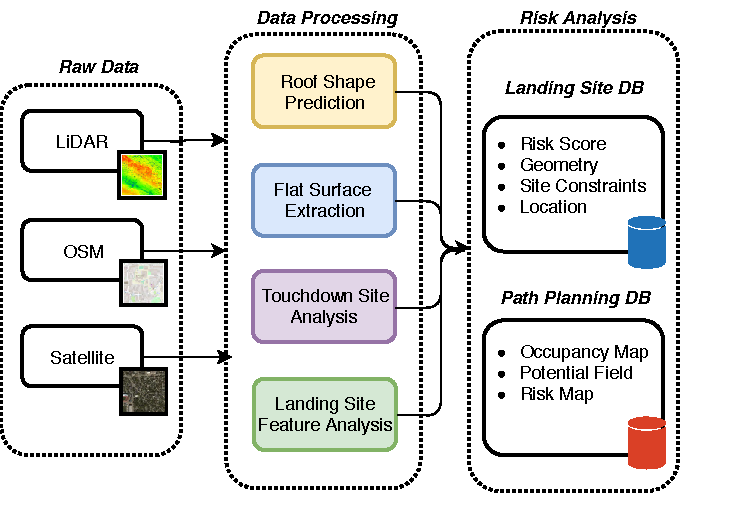
\includegraphics[clip, trim=0.0cm 0cm 0cm 0cm, width=0.6\linewidth]{chapter_5_mapping/imgs/data_preprocessing-Page-1.pdf}
    \caption{Data processing pipeline to construct landing site and occupancy map databases with risk values.}
    \label{fig:ch5_overview_processing}
\end{figure}


\paragraph{Landing Site Selection}
A set of candidate landing sites are generated within a radial footprint $R$
\begin{align}
    \mathcal{S}_{ls} = \{ l_i, \ldots, l_n \}
\end{align}
where each $l_i$ refers to a landing site with properties
\begin{align}
    l_i = \{ \mathbf{c},\; r_{l}, \;r_{p} \} \\
    \mathbf{c} \in \mathbb{R}^3 \\
    r_{l}, r_{p}  \in \mathbb{R} %\in [0,1]
\end{align}
where $\mathbf{c}$ is landing site location in a Cartesian reference frame, $r_{l}$ is landing site risk, and $r_{p}$ is path risk. Landing site risk is calculated offline and represents the risk intrinsic to touching down at that landing site. Path risk must be calculated online and accounts for the path distance and proximity to obstacles. A linear weighting scheme between the objectives is proposed below for each landing site $l_i \in \mathcal{S}_{ls} $:
\begin{equation}\label{eq:total_risk}
    r_{t} = w_l \cdot r_{l} + w_p \cdot r_{p}
\end{equation}
where $r_{t}$ refers to the total risk and $w_l$ and $w_p$ are weights for landing site risk and path risk, respectively. The optimal landing site can then be found by solving the optimization problem shown in Eq. \ref{eq:optimization}.
\begin{equation}
    l_{i^*} = \argminA_{l_i \; \in \; \mathcal{S}_{ls}} \; r_{t}\label{eq:optimization}
\end{equation}

A key insight into our multi-goal planner is that the minimum total risk $r_{t,min}$ of all landing sites can be calculated without computationally expensive path planning by using distance heuristics. The multi-goal planner can then prioritize searching for landing sites by lowest $r_{t,min}$ and halt search once a landing site's true total risk is less than all other sites' minimum total risk. 
% something I want to do later is paralleize this

\paragraph{Results}

An example case study in Witten is shown in Figure \ref{fig:ch5_ny_map1}. The position of the UAS is indicated by the green marker with nearby landing sites shown in color. Landing site risk is colorized from low (yellow) to high (dark orange) risk, with associated touchdown sites marked as blue circles. The lowest risk landing sites are ranked and marked with blue numbered icons. Our planner's chosen landing site is marked in red; this site balances landing site and path risk. Figure \ref{fig:ch5_ny_pareto} shows a Pareto plot demonstrating the trade off between landing site risk and path risk. Each purple dot represents risk for a landing site and its risk-optimal associated path, while the red dot signifies the planner's choice which minimizes total weighted risk. The green Pareto front connects the risk-optimal landing sites with respect to landing site and path risk.
% To generate these plots, collision-free paths to \textit{all} landing sites were generated, providing their actual path risk. 
% The $A^{*}$ path planning algorithm is used to search through occupancy maps to determine trajectories to landing sites and their associated path risk, $r_p$.
% Publicly available GIS data sources from the cities of Witten, Ann Arbor, and New York were processed to create risk-evaluated landing site databases and occupancy maps for path planning as outlined in Figure \ref{fig:ch5_overview_processing}. 

\begin{figure}
    \centering
    \begin{subfigure}[b]{0.44\linewidth}
        % \centering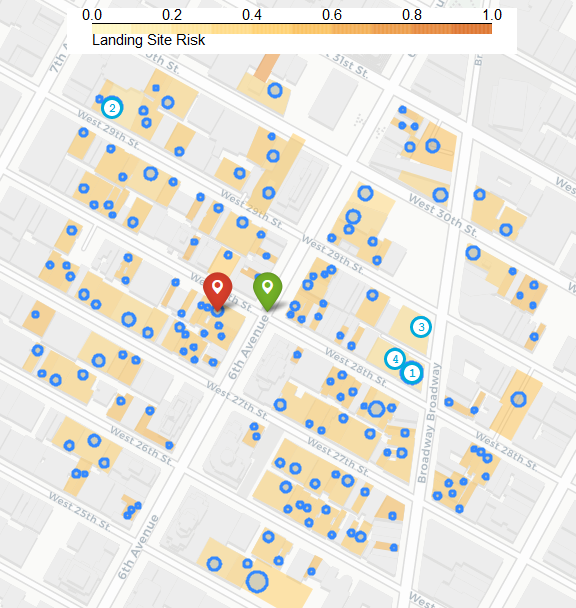
\includegraphics[clip, width=155pt, height=130pt]{chapter_5_mapping/imgs/newyork_scenario_1.png}
        \centering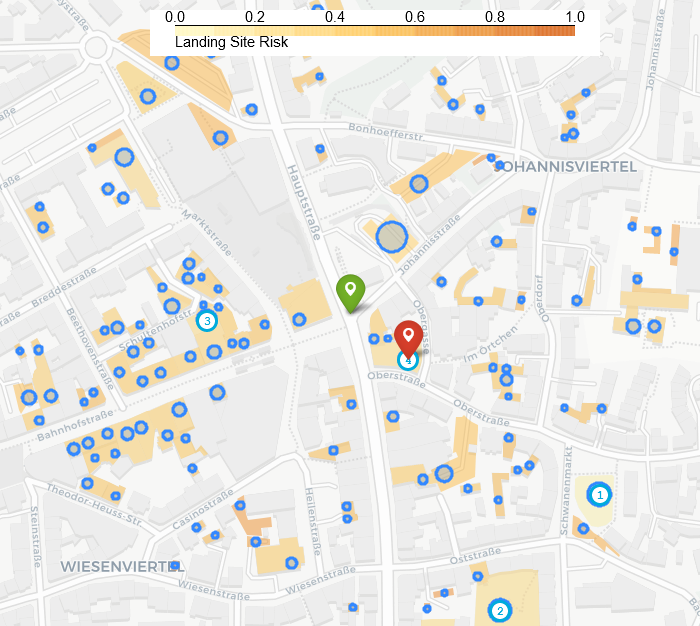
\includegraphics[clip, width=\linewidth, height=170pt]{chapter_5_mapping/imgs/witten_scenario_1.png}
        \caption{\label{fig:ch5_ny_map1}}
    \end{subfigure}
    \begin{subfigure}[b]{0.49\linewidth}
        % \centering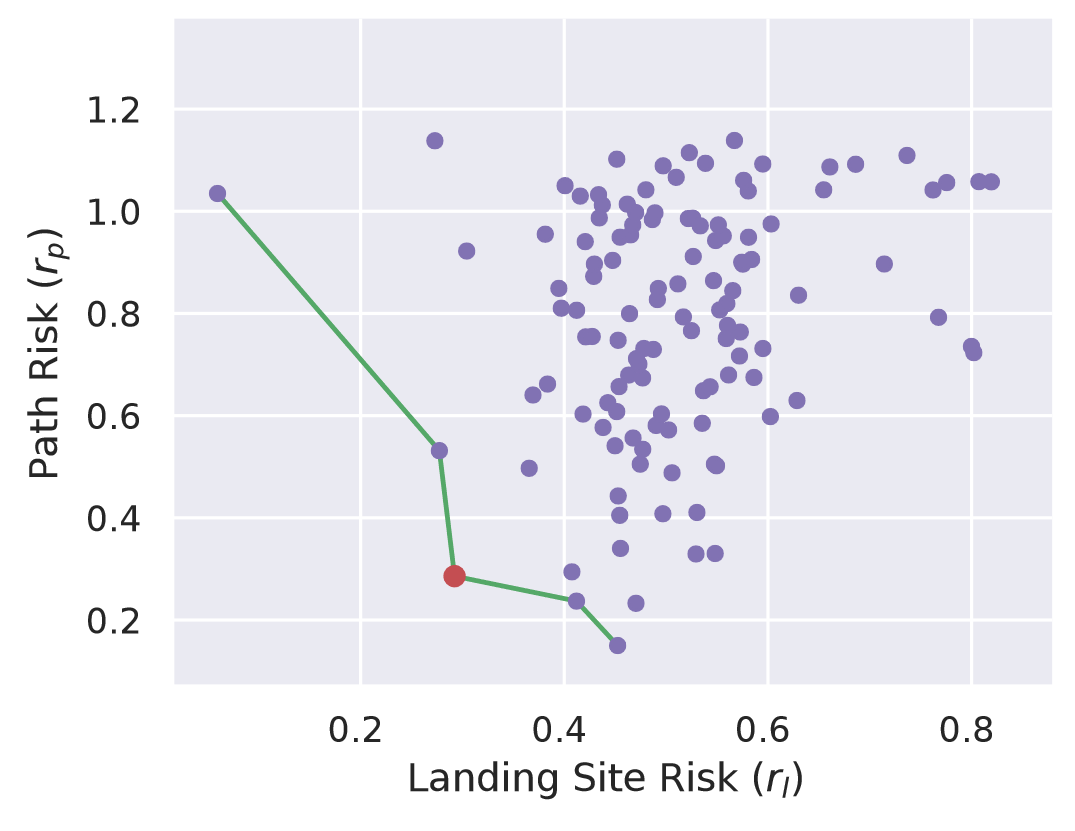
\includegraphics[clip, width=155pt, height=130pt]{chapter_5_mapping/imgs/PaertoFront.png}
        \centering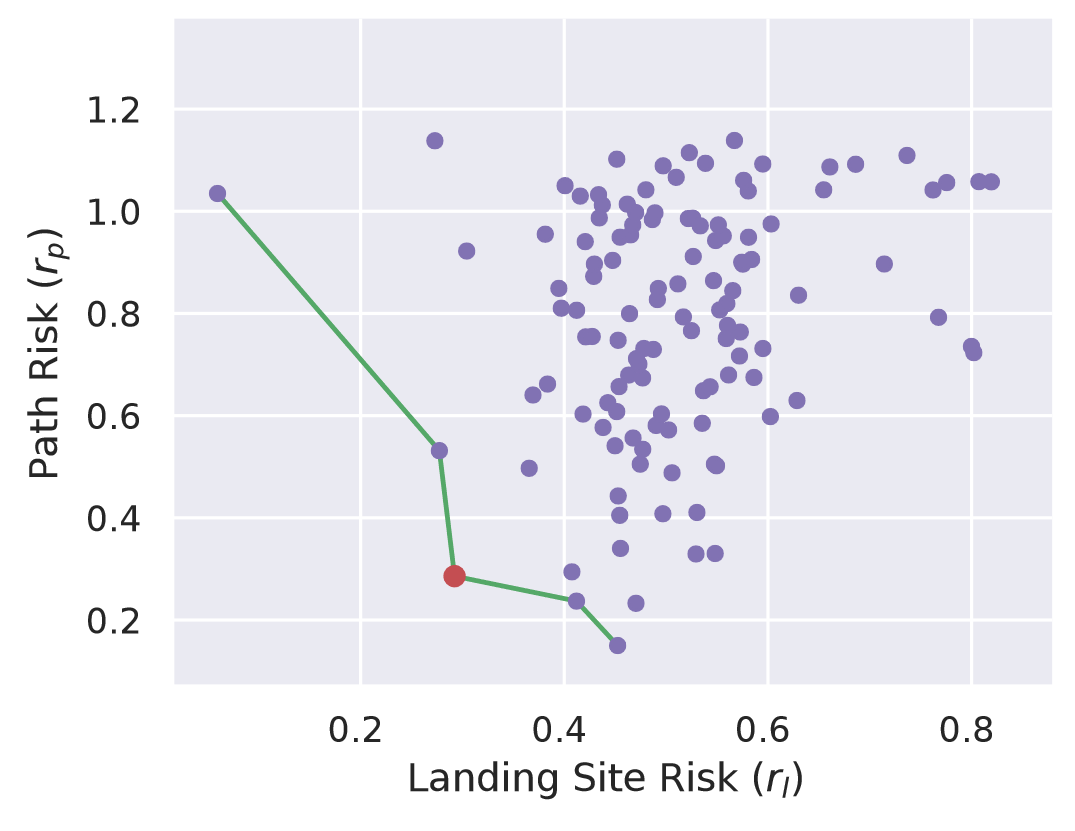
\includegraphics[clip, width=\linewidth, height=170pt]{chapter_5_mapping/imgs/PaertoFront.png}
        \caption{\label{fig:ch5_ny_pareto}}
    \end{subfigure}
    \caption{Urgent landing scenario in Manhattan New York. (\subref{fig:ch5_ny_map1}) Map of risk-evaluated landing sites (\subref{fig:ch5_ny_pareto}). Each purple dots represents a landing site and its associated path, while the red dot signifies the planner's choice that minimizes total weighted risk. }
    \label{fig:ch5_landing_site_selection}
\end{figure}


% \section{}

\paragraph{Conclusion}
This chapter demonstrates the use of nearby flat rooftops to augment traditional emergency landing sites such as parks and fields. Suitable rooftop surfaces are found by processing offline GIS data with roof shape identification and flat surface extraction with clear flat surfaces ultimately represented as polygons. Touchdown points for all terrain and rooftop surfaces are found by optimizing over distance to obstacles and calculating landing site risk. Landing site databases and 3D risk maps were generated for three diverse cities with results presented from six case studies with one example presented in this chapter summary. The multi-goal landing path planner minimizes a weighted sum of landing site and path risk for the UAS. A full description of all methods, risk models, and results can be found in our full paper \cite{castagno_map-based_2021}.
 
\chapter{Experimental Results for Real-time Landing Site Identification and Selection (Proposed)}
 \label{ch:experiments}
 % \section{Introduction}

This chapter will extend offline landing site identification and selection methods described previously to support real-time operation using on-board sensors. Small UAS carrying LiDAR, RGBD cameras, or monocular cameras using Structure from Motion (SfM) can generate 3D point clouds of nearby landing sites. Polylidar3D can transform these dense point clouds to polygonal representations of flat-surfaces in real-time while accounting for obstacles.  Alternatively, many point cloud scans may be integrated into a larger cohesive mesh in which noise is reduced. The final mesh can then be sent to Polylidar3D for polygon extraction. In either case a previously-defined final touchdown site can be validated as obstacle-free or a new site defined as the largest inscribed circle within the polygon can be identified.
In the coming months, we propose to conduct a series of experiments in which a flying UAS hovers over obstacle-laden flat surfaces in the M-Air netted facility. Our landing site selection procedure can then be tested in real-time. M-Air offers a motion capture system to provide ground truth of the environment to allow accuracy assessment. Multiple LiDAR/camera combinations will be evaluated.


\paragraph{Preliminary Results}

In August 2019 the author (Castagno) interned at the NASA Langley Research Center to conduct experiments related to landing site selection. A custom built drone frame was used with an onboard Pixhawk flight controller, Intel NUC companion board, and a 16-beam Velodyne Puck Lite LiDAR. The LiDAR sensor was mounted at $45^{\circ}$ underneath the drone and flights were conducted in an indoor VICON-equipped motion capture facility as well as outside in a netted area with no motion capture. The basic setup for the experiments was to place obstacles in front of the drone, fly to an altitude above ground of 3.5m, and validate landing site selection algorithms. Figure \ref{fig:ch6_experiment} demonstrates one of the nine flight experiments conducted (six indoors and three outside). All data was captured and retained for later processing with possible algorithmic refinement.

\begin{figure}[ht]
    \centering
    \begin{subfigure}[t]{0.45\linewidth}
        \centering
        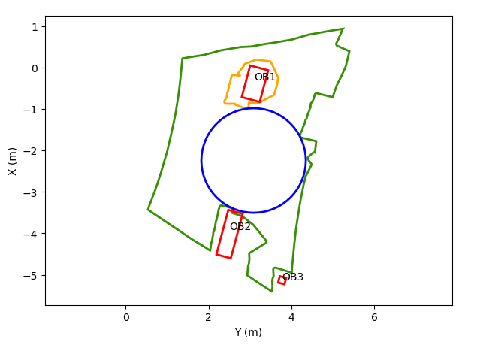
\includegraphics[width=0.99\textwidth]{chapter_6_experiments/imgs/experiments_1.pdf}
        \caption{}
        \label{fig:ch6_experiment_1}
    \end{subfigure}
    % \hfill
    \begin{subfigure}[t]{0.45\linewidth}
        \centering
        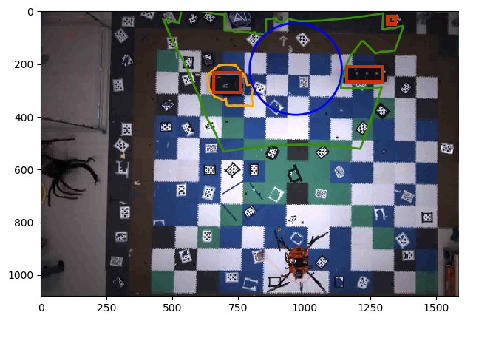
\includegraphics[width=0.99\textwidth]{chapter_6_experiments/imgs/experiments_2.pdf}
        \caption{}
        \label{fig:ch6_experiment_2}
    \end{subfigure}
    % \begin{subfigure}[t]{0.20\columnwidth}
    %     \centering
    %     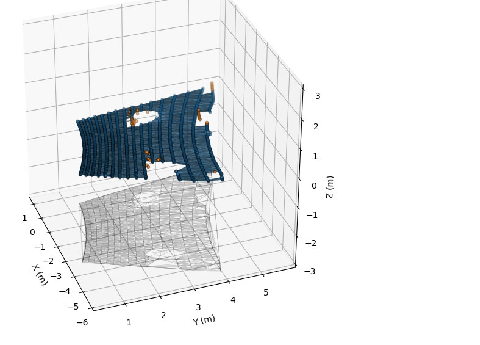
\includegraphics[trim=0cm 0cm 3cm 0cm, width=0.99\textwidth]{chapter_6_experiments/imgs/experiments_3.pdf}
    %     \caption{}
    %     \label{fig:ch6_experiment_3}
    % \end{subfigure}

    \caption{Landing site identification and selection from data collected at a NASA Langley facility. Obstacles positions are overlaid with red boxes. (a) Polylidar3D extracts a polygon of the surface represented as the the interior of the green polygon. The center of the blue circle is the selected touchdown point.  (b) Projection of all data onto an overhead camera.    }
    \label{fig:ch6_experiment}
    \hfill
\end{figure}

In real-time, every LiDAR scan was independently run through Polylidar3D and our selection algorithm.  In all cases the obstacles were captured accurately and a safe touchdown point was found. However there were cases ($\approx$ 5\%) where a stray LiDAR beam would cause a false positive causing non-optimal touchdown point selection. This motivated Polylidar3D refinment (already completed) to perform edge-preserving mesh smoothing and polygon filtering. Flight data captured at NASA Langley will be reprocessed with these updated Polylidar3D algorithms to guide future experiments.


\paragraph{Future Experiments}

Similar experiments will be performed in M-Air with different obstacle placements, sensor suites, lighting conditions, and potentially updates to Polylidar3D. We will primarily target use of a low-cost Intel RealSense L515 which is a \emph{solid state} LiDAR sensor. This device is significantly more lightweight (100 grams vs. 590+ grams) than a Velodyne unit and will offer a denser point cloud in the region of interest. We propose experiments where several elevated landing platforms will be placed in M-Air. Obstacles of varying size will be placed on these platforms. Different altitudes will tested, e.g., 3,6, and 9 meters above the ground.  Additionally instead of creating a mesh from a single scan,  multiple scans will be integrated to reduce noise using Truncated Signed Distance Function (TSDF) volume integration \cite{10.1145/237170.237269}. A final mesh will then be extracted with a marching cubes algorithm \cite{10.1145/37401.37422} and sent to Polylidar3D for flat surface extraction. 

\paragraph{Conclusion}

This chapter will extend offline landing site ID to an online (real-time) application supported by experimental validation.  Polylidar3D will extract flat surfaces from single scans and also from integrated meshes with multiple scans. A final journal publication will combine results from NASA and University of Michigan M-Air datasets.  We plan to submit results to the Journal of Field Robotics as well as a final dissertation chapter.








% \appendix

% \chapter{Proof of Optimality of Multi-Goal Planner}
%  \label{ch:proof_multi_goal}
%  Lots of talking here about planners and optimality

\section{Proof of Optimal Planner}



% \section{Lists Including the Appendices}
% The command
% \begin{verbatim}
% \showlistofappendices
% \end{verbatim}
% must appear in the preamble if there are more than one appendices.  For
% some reason, Rackham does not want the individual appendices and their
% sections to appear in the Table of Contents, so a special List of
% Appendices page (which must occur in the Table of Contents!) is required
% as a sort of extension to the Table of Contents.

% \nocite{*}


\bibliographystyle{aiaa}
\bibliography{thesis-bib}

\end{document}
